% === Dokumentklasse ==========================================================
\documentclass[%
    a4paper,							% A4
    12pt,								% Schriftgröße 12
    twoside,							% zweiseitig
    fleqn								% Formeln linksbündig ausrichten
]{book}


% === Grundlegende Pakete =====================================================
\usepackage{etoolbox}					% portiert viele nützliche Sachen aus e-TeX (z.B. booleans, ifs)
\usepackage[							% erweiterte Angabe von Farben
    pdftex,								% Farbtreiber auswählen
    dvipsnames							% vordefinierte Farben laden
]{xcolor}								% erweiterte Angabe von Farben
\usepackage{xparse}						% high-level Interface für Dokumentbefehle wie \NewDocument(Command,Environment)

\usepackage[utf8]{inputenc}				% Kodierung der *.tex Dateien ist UTF-8 nicht ISO-8859-1
\usepackage{cmap}						% character map tables -> pdf Inhalt wird besser durchsuch- und kopierbar
\usepackage[T1]{fontenc}				% OT1 encoding für deutsche Sonderzeichen -> pdf Inhalt kann Sonderzeichen durchsucht werden
\usepackage{lmodern}					% Latin-Modern-Schriftart (Computer Modern in Verbindung mit OT1 führt zu Bitmap-Fonts auf Windows)
\usepackage{microtype}					% mikrotypografische Einstellungen, die den gesetzten Text nochmals wesentlich verbessern (weniger badboxes)


% === Benutzerdefinierte Einstellungen ========================================
% === Art der Arbeit ==========================================================
% von den nachfolgenden Blöcken bitte den richtigen auswählen und die anderen auskommentieren/löschen

% --- Diplom ----------
%\newcommand{\settingsDegree}{{Diplom}}
%\newcommand{\settingsDegreeName}{{Diplominformatiker}}
%\newcommand{\settingsDegreeName}{{Diplomingenieur}}

% --- Bachelor ----------
% \newcommand{\settingsDegree}{{Bachelor}}
% \newcommand{\settingsDegreeName}{{Bachelor of Science}}

% --- Master ----------
\newcommand{\settingsDegree}{{Master}}
\newcommand{\settingsDegreeName}{{Master of Science}}

% === Name, Abgabedatum und Sprache der Arbeit ================================
\newcommand{\settingsName}{{Pierre Helbing}}
\newcommand{\settingsFinishDate}{{DD.MM.YYYY}}
\newcommand{\settingsLanguage}{german}   		% german / american

% === Weitere Einstellungen ===================================================
% --- Suchpfad (Unterverzeichnis) für eingebundene Grafiken ----------
\newcommand{\settingsGraphicsPath}{image/}

% --- Hinweiskapitel ----------
\newbool{settingsWithHints}
\setbool{settingsWithHints}{false}				% true / false

% --- Zeilennummern ----------
\newbool{settingsWithLineNumbers}
\setbool{settingsWithLineNumbers}{false}			% true / false

% --- Todos ----------
\newbool{settingsWithTodos}
\setbool{settingsWithTodos}{true}				% true / false

% --- Anzahl an Nummerierungsebenen im Text und Inhaltsverzeichnis ----------
% 1: \section
% 2: \section + \subsection
% Achtung: 3 oder 4 nur nach Absprache mit Betreuer !
% 3: \section + \subsection + \subsubsection
% 4: \section + \subsection + \subsubsection + \paragraph
\setcounter{secnumdepth}{2}
\setcounter{tocdepth}{2}

% --- Anforderungen ----------

\usepackage{tabularx}
\usepackage{multicol}
\newenvironment{myreq}[1]{%
    \setlist[description]{font=\normalfont\color{darkgray}}%
    \begin{tcolorbox}[colframe=black,colback=white, sharp corners, boxrule=1pt]%
        \bfseries\color{blue}%
        \begin{description}#1}%
            {\end{description}\end{tcolorbox}}

\newcommand{\threeinline}[3]{\begin{multicols}{3}#1 #2 #3\end{multicols}}
\newcommand{\twoinline}[2]{\begin{multicols}{2}#1 #2\end{multicols}}

\newcommand{\reqno}{\item[Requirement \#:]}
\newcommand{\reqtype}{\item[Requirement Type:]}
\newcommand{\reqevent}{\item[Event/BUC/PUC \#:]}
\newcommand{\reqdesc}{\item[Description:]}
\newcommand{\reqrat}{\item[Rationale:]}
\newcommand{\reqorig}{\item[Originator:]}
\newcommand{\reqfit}{\item[Fit Criterion:]}
\newcommand{\reqsatis}{\item[Customer Satisfaction:]}
\newcommand{\reqdissat}{\item[Customer Dissatisfaction:]}
\newcommand{\reqdep}{\item[Dependencies:]}
\newcommand{\reqconf}{\item[Conflicts:]}
\newcommand{\reqmater}{\item[Materials:]}
\newcommand{\reqhist}{\item[History:]}
\usepackage{multicol}
\usepackage{multirow}
\usepackage[dvipsnames]{xcolor}
\usepackage{enumitem}
\usepackage{tcolorbox}

% === Übersetzungen ===========================================================
% Definitionen je nach \mylanguage (siehe NIKR_settings.tex)
\ifdefstring{\settingsLanguage}{german}{%
    \newcommand{\acroname}{Abkürzungsverzeichnis}	% Name für Abkürzungsverzeichnis
    \newcommand{\todoname}{Todo Liste}	% Name für Todo-Liste
    \newcommand{\pagename}{Seite}		% Name für Seite
}%
{%
    \newcommand{\acroname}{Acronyms}	% Name für Abkürzungsverzeichnis
    \newcommand{\todoname}{Todo list}	% Name für Todo-Liste
    \newcommand{\pagename}{page}		% Name für Seite
}%


% === Wichtige Pakete und Einstellungen =======================================
\usepackage{calc}						% ermöglicht Arithmetik in den Argumenten von Befehlen

% Einstellungen je nach \mylanguage (siehe NIKR_settings.tex)
\ifdefstring{\settingsLanguage}{german}{%
    \usepackage[ngerman]{babel}			% Spracheinstellungen (für deutsch z.B. Contents -> Inhaltsverzeichnis, etc.)
    \usepackage{bibgerm}            	% Stylefile für deutsche Literaturstellenangabe
    \bibliographystyle{gerapali}		% Stil für Literaturangaben festlegen
}%
{%
    \usepackage[american]{babel}		% Spracheinstellungen (für deutsch z.B. Contents -> Inhaltsverzeichnis, etc.)
    \bibliographystyle{apalike}			% Stil für Literaturangaben festlegen
    \frenchspacing						% einfaches Leerzeiches nach Satzende (für deutsch bereits Standard)
}%
\usepackage[%
    noadjust							% noadjust verhindert automatische Leerzeichen um die Referenz, was am Zeilenanfang zu Problemen führt
]{cite}     							% erlaubt Zeilenumbruch innerhalb von Zitierungen

\usepackage{graphicx}					% erweiterte Argumente in \in­clude­graph­ics
\graphicspath{{\settingsGraphicsPath}}	% Standard-Pfad für Bilder siehe NIKR_settings.tex

\usepackage[bf]{caption}				% erlaubt erweiterte Formatierungen in \caption (siehe unten)
\usepackage{subcaption}					% mehrere Abbildungen nebeneinander

\usepackage{amsmath}					% ermöglicht \DeclareMathOperator
\usepackage{amssymb}					% mathmatische Symbole und Sonderzeichen
\usepackage{nicefrac}					% für \nicefrac
\usepackage{nccmath}					% für \mfrac

\usepackage{icomma}						% intelligentes Komma (macht Verwendung von {,} überflüssig)
\usepackage{siunitx}					% für einheitliche Angabe von Einheiten

\usepackage{fancyhdr}					% Kopf- und Fußzeilen (siehe unten)

\usepackage{hhline}						% erweitere Rahmengestaltung in Tabellen

\usepackage[%							% Einbettung von Links im Dokument und erlaubt die Nutzugn von \url
    hyperfootnotes=false,				% keine Fußnoten als Link im Dokument (geht nicht mit footmisc)
    pagebackref=true					% Backrefs im Literaturverzeichnis
]{hyperref}           					% Einbettung von Links im Dokument und erlaubt die Nutzugn von \url
\renewcommand*{\backref}[1]{\textit{(\pagename:~#1)}}   % Format für backrefs

\usepackage[%							% erlaubt erweiterte Formatierungen von Fußnoten (siehe unten)
    multiple,							% mehrere mit Komma abtrennen
    hang								% linksbündig, \footnotemargin entscheidet über Einrückung
]{footmisc}								% erlaubt erweiterte Formatierungen von Fußnoten (siehe unten)
\patchcmd{\footref}{\ref}{\ref*}{}{}	% Hyperlink in \footref entfernen

\usepackage[nohyperlinks]{acronym}		% Abkürzungsverzeichnis

\usepackage{setspace}					% für \setstretch (ändern Zeilenabstand, aber nicht floating Umgebungen)

\usepackage[%							% Todos
    colorinlistoftodos,					% farbige Markierungen in Todo-Liste
    prependcaption,						% caption=val
    textsize=tiny,						% Schriftgröße
    linecolor=red,						% Standard-Linienfarbe für \todo
    backgroundcolor=red!25,				% Standard-Hintergrundfarbe für \todo
    bordercolor=red,					% Standard-Rahmenfarbe für \todo
    textwidth=2cm,						% Standard-Breite für \todo
]{todonotes}							% Todos
\ifbool{settingsWithTodos}{%
    \setlength{\marginparwidth}{2cm}	% sonst werden Notes am Rand nicht richtig angezeigt
    \NewDocumentCommand{\todoaddref}{O{} m}{%
        \todo[linecolor=blue,backgroundcolor=blue!25,bordercolor=blue,#1]{#2}%
    }
    \NewDocumentCommand{\todouncertain}{O{} m}{%
        \todo[linecolor=green,backgroundcolor=green!25,bordercolor=green,#1]{#2}%
    }
    \NewDocumentCommand{\todooptional}{O{} m}{%
        \todo[linecolor=cyan,backgroundcolor=cyan!25,bordercolor=cyan,#1]{#2}%
    }
    \pretocmd{\mainmatter}{\listoftodos[\todoname]{\markboth{\MakeUppercase{\todoname}}{\MakeUppercase{\todoname}}}}{}{}
}{
    \presetkeys{todonotes}{disable}{}	% disable \todo
    \NewDocumentCommand{\todoaddref}{O{} m}{}
    \NewDocumentCommand{\todouncertain}{O{} m}{}
    \NewDocumentCommand{\todooptional}{O{} m}{}
}

\usepackage[switch*,pagewise]{lineno}	% Zeilennummern
\ifbool{settingsWithLineNumbers}{%
    \renewcommand\linenumberfont{\textbf\sffamily\color{black!50}\footnotesize}
    \apptocmd{\mainmatter}{\linenumbers}{}{}
    \pretocmd{\backmatter}{\nolinenumbers}{}{}
}{}

\usepackage{placeins}					% FloatBarriers

\usepackage{enumitem}					% erweiterte Formatierung von \enumerate, \itemize und \description

\usepackage[linewidth=0.5pt]{mdframed}	% für Boxen in Hinweisen

\usepackage[ddmmyyyy]{datetime}			% Datumsangabe
\renewcommand{\dateseparator}{.}		% Punkt als Trennzeichen in Datumsangabe


% === Längen und Abstände =====================================================
% horizontales Layout
\setlength{\oddsidemargin}{0.2in}
\setlength{\evensidemargin}{0.0in}
\setlength{\textwidth}{\paperwidth - 2.2in}

% vertikales Layout
%\setlength{\topskip}{0.0cm}
\setlength{\headheight}{15.1pt}
%\setlength{\headsep}{0.0cm}
\setlength{\topmargin}{0.0cm}
\setlength{\footskip}{0.6in}
\setlength{\textheight}{\paperheight - 2.0in}
\addtolength{\textheight}{-1.0\headheight}
\addtolength{\textheight}{-1.0\headsep}
\addtolength{\textheight}{-1.0\footskip}

% Zeilenabstand
\setstretch{1.3}
\AtBeginEnvironment{tabular}{\setstretch{1.3}}

% Einrückung von Formeln
\setlength{\mathindent}{1.0cm}

% Absätze
\setlength{\parindent}{0.0cm}

% Fußnoten
\renewcommand{\footnotelayout}{\setstretch{1.2}}
\setlength\footnotemargin{10pt}

% Listen (noitemsep, nosep, ...)
\setlist{noitemsep}

\setlength{\topsep}{0.3cm}


% === Bild- und Tabellenunterschrift ==========================================
\renewcommand{\captionfont}{\small \setstretch{1.3}}
\newcommand{\NIcaption}[2]{\caption[#1]{#1\protect\\ \emph{#2}}}
\setcaptionmargin{0.75cm}


% === Abkürzungsverzeichnis ===================================================
% Verwendung vor jedem Kapitel zurücksetzen
\pretocmd{\chapter}{\acresetall}{}{}


% === Seitenstil ==============================================================
% Pagestyle plain überschreiben
\pagestyle{fancy}
% Kapitel- und Abschnittangaben ohne Punkt
\renewcommand{\sectionmark}[1]{\markright{\uppercase{\thesection~~#1}}}
\renewcommand{\chaptermark}[1]{\markboth{\uppercase{\chaptername\ \thechapter~~#1}}{}}
\fancypagestyle{plain}{%
    \fancyhead[ER]{\itshape\leftmark}%
    \fancyhead[OL]{\itshape\rightmark}%
    \fancyhead[EL,OR]{\thepage}%
    \fancyfoot[EL,OL]{}%
    \fancyfoot[EC,OC]{}%
    \renewcommand{\headrulewidth}{0.4pt}%
    \renewcommand{\footrulewidth}{0.4pt}%
}


% === Verweise ================================================================
% Klammern in Formel-Referenzen entfernen
\makeatletter
\renewcommand\tagform@[1]{\maketag@@@{\ignorespaces#1\unskip\@@italiccorr}}
\makeatother


% === Angabe von Einheiten ====================================================
\ifdefstring{\settingsLanguage}{german}{%
    \sisetup{locale=DE}		% deutsche Lokalisierung (konvertiert 1.00 automatisch zu 1,00)
}%
{%
    \sisetup{locale=US}		% englische Lokalisierung (konvertiert 1,00 automatisch zu 1.00)
}%


% === Mathematische Definitionen ==============================================
% Darstellung von Vektoren und Matrizen
\renewcommand{\vec}[1]{\underline{\mathbf{\MakeLowercase{#1}}}}		% Vektoren
\newcommand{\veci}[1]{\underline{\MakeLowercase{#1}}}				% Vektoren als Indizes
\newcommand{\mat}[1]{\underline{\mathbf{\MakeUppercase{#1}}}}		% Matrizen
\newcommand{\mati}[1]{\underline{\MakeUppercase{#1}}}				% Matrizen als Indizes
% zusätzliche mathematische Operatoren (damit sie nicht als Formelzeichen geschrieben werden)
\DeclareMathOperator{\step}{step}									% Stufenfunktion
\DeclareMathOperator{\sign}{sign}									% Vorzeichen


% === Manuelle Definition von Worttrennungen ==================================
\hyphenation{
    Convolutional
    Neural
    Net-work
    Net-works
    Ko-ef-fi-zi-ent
    Ko-ef-fi-zi-ent-en
    Drop-out
    pixel-genaue
    Patch
    Patch-größen
}


% === Pseudocode-Darstellung ==================================================
% Import nicht oben, weil \parindent zuvor gesetzt werden muss!
% siehe: https://ctan.org/pkg/algorithm2e?lang=de
\ifdefstring{\settingsLanguage}{german}{%
    \usepackage[%						% Pseudocode
        linesnumbered,					% mit Zeilennummern
        noend,							% Ende von Befehlen, wie etwa While, unterdrücken
        ruled,							% Layout
        german,							% deutsche Bezeichnung und deutsches Verzeichnis
        %onelanguage,					% Keywords übersetzen
        algochapter						% Nummerierung analog zu Abbildungen
    ]{algorithm2e}						% Pseudocode
}{%
    \usepackage[%						% Pseudocode
        linesnumbered,					% mit Zeilennummern
        noend,							% Ende von Befehlen, wie etwa While, unterdrücken
        ruled,							% Layout
        algochapter						% Nummerierung analog zu Abbildungen
    ]{algorithm2e}						% Pseudocode
}%

\newenvironment{NIalgorithm}{%
    % Algorithmus um 1.5em einrücken, damit Zeilennummern nicht im Rand sind
    \setlength{\algomargin}{1.5em}%
    % Padding oben und unten für Caption
    \setlength{\interspacetitleruled}{\smallskipamount}%
    % Padding oben und unten für Algorithmus
    \SetAlgoInsideSkip{smallskip}%
    % Kommentarstyle ändern
    \newcommand\NIcommentstyle[1]{\ttfamily\textcolor{black!60}{##1}}
    \SetCommentSty{NIcommentstyle}%
    % zweiten Teil in NIcaption unterdrücken (falls NIcaption genutzt wird)
    \renewcommand{\NIcaption}[2]{\caption[##1]{##1}}%
    \begin{algorithm}%
        % Zeilenabstand minimal vergrößern
        \setstretch{1.1}%
        % kleine Schrift
        \small%
        % Semikolon unterdrücken
        \DontPrintSemicolon%
        % korrekt ausgerichtete mehrzeilige Input- bzw. Outputdefinitionen mittels \Input und \Output
        \SetKwInOut{Input}{Input}%
        \SetKwInOut{Output}{Output}%
        % Abschnitt für In- und Outputs zurückrücken
        \pretocmd{\Input}{\Indentp{-1.5em}}{}{}%
        \apptocmd{\Output}{\Indentp{1.5em}}{}{}%
        }{%
    \end{algorithm}%
}

\begin{document}
% --- Titelseite, Danksagung, Einverständniserklärung --------------------------
\pagestyle{empty}
% Buchstaben für Seitennummerierung verwenden 
% (verhindert "destination with the same identifier (name{page.X})" Warnung)
\pagenumbering{alph}

% === Titelblatt ==============================================================
\begin{titlepage}
	\hspace{0.2cm}
	\begin{minipage}{3.5cm}
		
\includegraphics[width=0.8\textwidth]{images/logo}
	\end{minipage}
	\hspace{0.2cm}
	\begin{minipage}{11cm}
		\vspace{0.7cm}
		\large
		{\bf Technische Universität Ilmenau}\newline
		Fakultät für Informatik und Automatisierung\newline
		Fachgebiet Neuroinformatik und Kognitive Robotik
	\end{minipage}
	\begin{center}
		\vspace{0.8cm}
		{\Large\bfseries Entwicklung einer CrossLab-kompatiblen integrierten Entwicklungsumgebung für das GOLDi-Remotelab\\}
		\vspace{0.8cm}
		\settingsDegree arbeit zur Erlangung des akademischen Grades \settingsDegreeName\\[0.5cm]
		{\Large \bfseries \settingsName\\[1.0cm]}
		\begin{table}[ht]
			\centering
			\begin{tabular}{ll}
				Betreuer: & Dr. Detlef Streitferdt                    \\[2mm]
				\multicolumn{2}{l}{Verantwortlicher Hochschullehrer:} \\
				          & Prof. Dr.-Ing. habil. Daniel Ziener       \\[2cm]
				\multicolumn{2}{p{13cm}}{Die \settingsDegree arbeit wurde am \settingsFinishDate \ bei der Fakultät für Informatik und Automatisierung der Technischen Universität Ilmenau eingereicht.}
			\end{tabular}
		\end{table}
		% Hinweis für Entwurfsversion ausgeben (Variablen aus NIKR_settings.tex prüfen)
		\ifboolexpr{bool{settingsWithTodos} or bool{settingsWithLineNumbers} or bool{settingsWithHints}}{%
		{\color{red} Entwurf: \today \\[2mm]
		\textbf{Dies ist nicht die finale Druckvorlage.}\\[2mm]
		{\small%
		\ifbool{settingsWithHints}{%
			Hinweiskapitel aktiviert (siehe \texttt{settingsWithHints} in \texttt{NIKR\_settings.tex})\\%
		}{}%					
		\ifbool{settingsWithLineNumbers}{%
			Zeilennummern aktiviert (siehe \texttt{settingsWithLineNumbers} in \texttt{NIKR\_settings.tex})\\%
		}{}%
		\ifbool{settingsWithTodos}{%
			Todo-Markierungen aktiviert (siehe \texttt{settingsWithTodos} in \texttt{NIKR\_settings.tex})\\%
		}{}%
		}%
		}%
		}{}
	\end{center}
\end{titlepage}

\cleardoublepage

% === Danksagung ==============================================================
% Sollten Sie diesen Abschnitt nicht nutzen wollen, kommentieren Sie alle Zeilen
% bis zur Einverstaendniserklaerung (inkl. \cleardoublepage) aus
\vspace*{5cm}

Danksagung

Dieser Abschnitt {\bf kann} genutzt werden, um denjenigen Personen Dank auszusprechen, die Sie bei der Erstellung der Arbeit unterstützt haben.

\cleardoublepage

% === Einverstaendniserklaerung ================================================
\vspace*{16cm}

\begin{tabular}{lp{12.5cm}}
	{Erklärung:} & {"`Hiermit versichere ich, dass ich diese wissenschaftliche Arbeit selbständig verfasst und nur die angegebenen

			
			
			
			
			
			
			
			
			
			
			Quellen und Hilfsmittel verwendet habe. Alle von mir aus anderen
			Veröffentlichungen übernommenen Passagen sind als solche gekennzeichnet."'}
\end{tabular}
\vspace*{1.5cm}

\begin{tabular}{l}
	Ilmenau, \settingsFinishDate \\
	\\
\end{tabular}
\hfill
\begin{tabular}{c}
	{\makebox[6.0cm]{\dotfill}} \\
	\settingsName               \\
\end{tabular}

\cleardoublepage


% --- Inhalts- und Abkürzungsverzeichnis ---------------------------------------
\frontmatter
\pagestyle{plain}
% Inhaltsverzeichnis
\tableofcontents
% Abkürzungsverzeichnis
\chapter*{\acroname}
\markboth{\MakeUppercase{\acroname}}{\MakeUppercase{\acroname}}
% 1. Definition von Abkürzungen
\begin{acronym}[XXXXXX] % durch XXXXXX kann der Einzug bestimmt wird
	\setlength{\itemsep}{-\parsep}
	\acro{IDE}{Integrated Development Environment}
	\acro{LSP}{Language Server Protocol}
	\acro{DAP}{Debug Adapter Protocol}
	\acro{VSCode}{Visual Studio Code}
	\acro{OT}{Operational Transformation}
	\acro{CRDTs}{Conflict-free Replicated Data Types}
	\acro{LMS}{Lernmanagementsysteme}
	\acro{LTI}{Learning Tools Interoperability}
\end{acronym}

% 2. Beispiel für Verwendung im Fließtext, z.B.: \ac{CNN}



% --- Inhalt -------------------------------------------------------------------
\mainmatter

% Hinweiskapitel
\ifbool{settingsWithHints}{\input{content/hinweise}}{}

% Kapitel
\chapter{Einleitung}\label{section:einleitung}

\begin{note}
    \textbf{Notizen:}
    \begin{itemize}
        \item Remote Labore (z.B. GOLDi)
        \item IDEs in Remote Laboren (z.B. GOLDi und WIDE)
        \item Änderungen und Möglichkeiten durch CrossLab
        \item Weiterer Verlauf der Arbeit
    \end{itemize}
\end{note}
\todo{Einleitung}

% Das Grid of Online Laboratory Devices Ilmenau (GOLDi) ist ein hybrides Online Labor. Es ermöglicht Studierenden reale sowie simulierte elektromechanische Hardwaremodelle mit verschiedenen Kontrolleinheiten zu steuern. Vor dem CrossLab Projekt waren nur Experiment mit einem Hardwaremodell und einer Kontrolleinheit möglich. Aufgrund der neuen CrossLab Architektur ist es allerdings nun möglich Experimente freier zu konfigurieren. Dabei werden sogenannte Laborgeräte definiert, die gewisse Services anbieten. Über diese Services können verschiedene Laborgeräte zu einem Experiment zusammengefügt werden. Nehmen wir zum Beispiel ein 3-Achs-Portal sowie einen Microcontroller. Beide diese Geräte können einen Service anbieten, der ihre Pins definiert. Über diese Services können dann die Pins der beiden Geräte verbunden werden.

% WIDE ist eine eigens für das GOLDi Remotelab entwickelte integrierte Entwicklungsumgebung (IDE). Sie ermöglicht es Nutzern direkt im Browser Programme für die Kontrolleinheiten zu schreiben. Weiterhin wird auch die Kompilierung des Quellcodes sowie das Hochladen des Kompilats auf die Kontrolleinheit unterstützt. Allerdings ist WIDE auf die alte Architektur des GOLDi Remotelab ausgelegt, in welcher ein Experiment nur aus jeweils einem Hardwaremodell und einer Kontrolleinheit bestand. In der neuen CrossLab Architektur kann jedoch ein Experiment mehrere Hardwaremodelle und Kontrolleinheiten enthalten.

% Um die neuen Anforderungen, die aus der CrossLab Architektur hervorgehen, zu addressieren ist eine Anpassung bzw. Neukonzeption von WIDE nötig. Dafür werden in Kapitel \ref{grundlagen} einige grundlegende Begriffe eingeführt. Danach wird in Kapitel \ref{systematische_literaturrecherche} eine Systematische Literaturrecherche durchgeführt. In Kapitel \ref{anforderungsanalyse} werden die Anforderungen an eine IDE im Kontext des GOLDi Remotelab sowie der CrossLab Architektur gesammelt. In Kapitel \ref{stand_der_technik} werden bestehende Lösungen auf ihre Anwendbarkeit überprüft und verglichen. In Kapitel \ref{konzeption} wird die Lösung konzipiert. In Kapitel \ref{implementierung} wird die Implementierung der konzipierten Lösung beschrieben. In Kapitel \ref{auswertung} wird der Erfüllungsgrad der Anforderungen ausgewertet. Schließlich wird in Kapitel \ref{zusammenfassung_und_fazit} eine Zusammenfassung der Arbeit sowie ein Fazit gegeben.
\chapter{Grundlagen}\label{section:grundlagen}

In diesem Kapitel werden einige Grundlagen für diese Arbeit beschrieben. Zunächst werden integrierte Entwicklungsumgebungen in \autoref{section:grundlagen:integrierte-entwicklungsumgebung} erläutert. Daraufhin werden das Verbundprojekt CrossLab und die dazugehörige Architektur für online Labore in \autoref{section:grundlagen:crosslab} vorgestellt.

\section{Integrierte Entwicklungsumgebung}\label{section:grundlagen:integrierte-entwicklungsumgebung}
Eine integrierte Entwicklungsumgebung bzw. \ac{IDE} ist meistens auf einen speziellen Anwendungsfall ausgelegt und besteht aus einem Code Editor sowie weiteren benötigten Softwarewerkzeugen, wie z.B. Compiler, Debugger und Language Server \cite{noauthor_language-server-protocol_nodate}. Dabei werden oftmals alle diese Komponenten direkt mit der \ac{IDE} ausgeliefert, wodurch der Nutzer direkt mit der Programmierung beginnen kann. Somit besitzt eine \ac{IDE} mehr Features als ein Code Editor, da diese nur die Bearbeitung von Code erlauben, während \acp{IDE} u.a. auch die Kompilierung und das Debuggen von Programmen ermöglichen. Language Server erweitern die Funktionen eines Code Editors, indem sie u.a. Code-Vervollständigung, Code-Navigation und Refactoring ermöglichen.

\section{CrossLab}\label{section:grundlagen:crosslab}
CrossLab \cite{aubel_adaptable_2022} ist ein Verbundprojekt der Technischen Universität Bergakademie Freiberg, der Technischen Universität Dortmund, der NORDAKADEMIE und der Technischen Universität Ilmenau. Im Rahmen des Projekts wurde eine neue Architektur für online Labore erarbeitet \cite{nau_new_2022}.

Die CrossLab-Architektur basiert auf dem Konzept von sogenannten \textit{Laborgeräten}. Diese können verschiedene \textit{Services} anbieten bzw. konsumieren. Beispiele für Services sind der \textit{Electrical Connection Service}, welcher den Austausch von Sensor- und Aktorwerten ermöglicht, und der \textit{Webcam Service}, welcher die Übertragung der Webcamaufnahmen von z.B einem elektromechanischen Hardwaremodell ermöglicht. Services besitzen immer einen \textit{Producer}, der die Funktionen des Services bereitstellt, sowie einen \textit{Consumer}, der diese nutzen kann. Dabei können auch sogenannte \textit{Prosumer} entwickelt werden, die beide Rollen erfüllen können. Durch die Verbindung der Services von verschiedenen Laborgeräten kann ein \textit{Experiment} erstellt werden. Ein Vorteil dieser Architektur ist die einfache Wiederverwendbarkeit und Austauschbarkeit von einzelnen Laborgeräten in Experimenten. So können z.B. Laborgeräte mit gleichen Services in einer entsprechenden \textit{Laborgerätegruppe} hinterlegt werden, welche dann statt eines konkreten Laborgeräts zur Erstellung eines Experiments genutzt werden kann. Beim Start des Experiments wird dann ein verfügbares Laborgerät aus der Laborgerätegruppe ausgewählt. Weiterhin gibt es noch \textit{cloud-instanziierbare} und \textit{edge-instanziierbare} Laborgeräte. Beim Start eines Experiments mit cloud- oder edge-instanziierbaren Laborgeräten wird eine entsprechende Instanz des Laborgeräts erstellt. Dabei wird für cloud-instanziierbare Laborgeräte eine Nachricht an die hinterlegte Instanziierungs-URL geschickt, wodurch die Instanz erstellt wird. Für edge-instanziierbare Laborgeräte wird mithilfe der hinterlegten Code-URL eine URL erstellt, die vom Nutzer aufgerufen werden muss um die Instanz zu erstellen.

Das Backend von CrossLab besteht aus mehreren verschiedenen Diensten, welche zusammen eine \textit{CrossLab-Instanz} bilden. Diese Dienste sind im Folgenden aufgelistet:
\begin{itemize}
    \item \textbf{Authentication Service} \\ Dieser Dienst ist für die Authentifizierung der Nutzer verantwortlich.
    \item \textbf{Authorization Service} \\ Dieser Dienst ist für die Authorisierung der Nutzer verantwortlich.
    \item \textbf{Device Service} \\ Dieser Dienst verwaltet die Laborgeräte der CrossLab-Instanz.
    \item \textbf{Experiment Service} \\ Dieser Dienst ist für die Erstellung und Verwaltung der Experimente der CrossLab-Instanz verantwortlich.
    \item \textbf{Federation Service} \\ Dieser Dienst ist für das Teilen von Laborgeräten und Experimenten mit anderen CrossLab-Instanzen verantwortlich.
\end{itemize}
Um ein Experiment in einer CrossLab-Instanz starten zu können benötigen Nutzer ein entsprechendes Nutzerkonto für diese CrossLab-Instanz.
\chapter{Stand der Technik} \label{stand-der-technik}

In diesem Kapitel soll der Stand der Technik dargestellt werden. Dazu wird zunächst in Abschnitt \ref{stand-der-technik-literaturrecherche} eine systematische Literaturrecherche durchgeführt und die Ergebnisse dieser geschildert.

\section{Literaturrecherche} \label{stand-der-technik-literaturrecherche}

Um einen Überblick über den aktuellen Stand der Forschung zu bekommen wird zunächst eine Literaturrecherche vorgenommen. Dabei sollen vorhandene online IDEs gefunden sowie die folgenden Fragen beantwortet werden:

\begin{itemize}
    \item Welche Implementierungen von online IDEs gibt es?
    \item Welchen Architekturmustern folgen online IDEs?
    \item Welche Vor- und Nachteile haben die online IDEs?
    \item Welche Anforderungen werden an online IDEs gestellt?
\end{itemize}

Die folgenden Datenbanken wurden für die Literaturrecherche ausgewählt:

\begin{itemize}
    \item ACM Digital Library
    \item IEEE Xplore
    \item Scopus
    \item Web of Science
\end{itemize}

Zunächst wurde eine allgemeine Suche nach online IDEs in den genannten Datenbanken vorgenommen. Dazu werden zunächst die in \autoref{table:search-terms} genannten Stichwörter jeweils mit ihren Synonymen mit einer OR-Operation verknüpft. Danach werden die daraus resultierenden Terme mit einer AND-Operation verbunden. Die so entstehende Suchanfrage werden dann für die Suche in den Datenbanken verwendet. Dabei werden die Titel, Abstracts und Keywords der Publikationen durchsucht.

In \autoref{table:amount-search-results} ist die Anzahl der Treffer für den einzelnen Datenbanken dargelegt. Um die Anzahl der zu betrachtenden Publikationen zu verringern wird eine weitere Filterung der Ergebnisse vorgenommen. Dafür werden nur Publikationen betrachtet, die IDE oder ein entsprechendes Synonym in ihrem Titel oder ihren Keywords enthalten. Dadurch sinkt die Anzahl der Treffer auf insgesamt $1705$. Danach werden alle exakten Duplikate über einen Vergleich der Titel und Links herausgefiltert wodurch die Anzahl der Publikationen auf $1243$ sinkt. In einem weiteren Schritt werden die Titel und Abstracts der Publikationen genauer betrachtet. Dabei werden unter anderem Arbeiten herausgefiltert, deren Titel und Abstracts keinen Bezug zu den Forschungsfragen besitzen. Weiterhin werden Publikationen bevorzugt, die sich zudem mit textbasierten Programmiersprachen, Kollaboration und Lehre auf Universitätsniveau befassen. Aus dieser Filterung resultieren $97$ Publikationen. Als letzte Filterung werden Publikationen, welche vor $2019$ veröffentlicht wurden aussortiert, falls sie weniger als $10$ Zitationen haben sowie vor $2014$ veröffentlichte Publikationen mit weniger als $25$ Zitationen. Die Anzahl der Zitationen wurde mithilfe von Google Scholar ermittelt. Dadurch ergibt sich die Anzahl von $64$ zu betrachtenden Publikationen.

\begin{table}[tbp]
    \centering
    \begin{tabularx}{\textwidth}{| >{\hsize=.6\hsize\linewidth=\hsize}X |
            >{\hsize=1.4\hsize\linewidth=\hsize}X |}
        \hline
        Stichwort                           & Synonyme                                                                                                     \\
        \hline
        integrated development environments & IDEs, code editors, development environments, development tools, programming tools, programming environments \\
        \hline
        web                                 & browser, online, cloud                                                                                       \\
        \hline
    \end{tabularx}
    \caption{Suchbegriffe}
    \label{table:search-terms}
\end{table}

\begin{table}[tbp]
    \centering
    \begin{tabular}{|c|c|c|c|c|c|}
        \hline
        ACM & IEEE & Scopus & Web of Science \\
        \hline
        785 & 1472 & 4661   & 1044           \\
        \hline
    \end{tabular}
    \caption{Anzahl Suchergebnisse}
    \label{table:amount-search-results}
\end{table}

\begin{figure}[htbp]
    \centering
    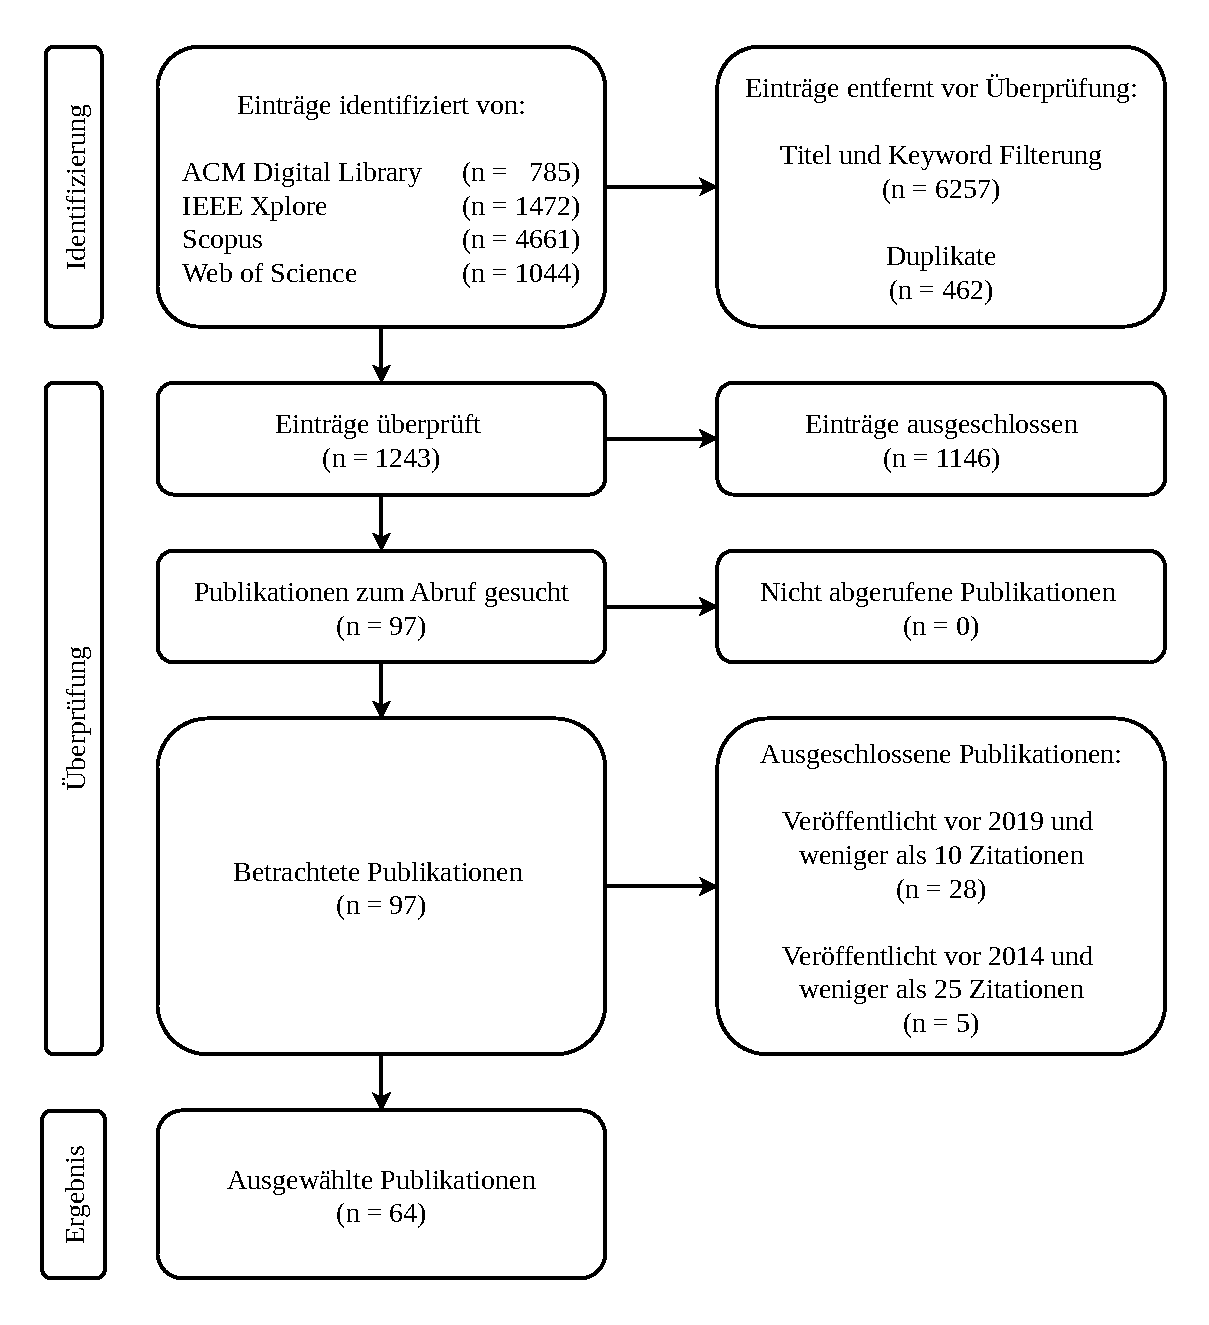
\includegraphics[width=\textwidth]{diagrams/PRISMA.pdf}
    \caption{PRISMA Diagramm}
    \label{prisma-diagram}
\end{figure}

Die Publikationen beschreiben eine Vielzahl an verschiedenen webbasierten integrierten Entwicklungsumgebungen. Dabei kann eine Unterteilung in die folgenden zwei Kategorien erfolgen:

\begin{itemize}
    \item \textbf{Client-Server-basierte Lösungen} \\
          Systeme dieser Art zeichnen sich dadurch aus, dass sie eine Client-Server-Archi-tektur verwenden. Hierbei werden Features, die nicht innerhalb eines Browsers ausgeführt werden können (z.B. Kompilierung) über einen entsprechenden Server bereitgestellt.
    \item \textbf{Browser-basierte Lösungen} \\
          Systeme dieser Art zeichnen sich dadurch aus, dass alle Features im Browser des Nutzers ausgeführt werden können, ohne die Hilfe eines separaten Servers.
\end{itemize}

Deursen et al. (2010) \cite{van_deursen_adinda_2010} beschreiben eine online IDE names Adinda. Die grundlegende Idee von Adinda ist die Zerlegung der Funktionalität einer IDE in einen leichtgewichtigen Client sowie mehrere zusammenarbeitende (Web-)Services. Diese Services sollen dann bestimmte Aufgaben erfüllen, wie z.B. Kompilierung, Testen, kollaboratives Editieren und Datenerhebung. Es werden weiterhin verschiedenste Forschungsfragen aufgestellt, die für das vorgestellte System von Interesse sind. Die prototypische Implementierung von Adinda basiert auf WWWorkspace \cite{ryan_web_2007} und nutzt serverseitig Eclipse \cite{noauthor_eclipse_nodate}. Der Prototyp unterstützt das Erstellen von Nutzer-Workspaces, Java Projekten, Paketen und Klassendateien sowie Syntax Highlighting, Kompilierung und Code-Vervollständigung. \todo{Adinda}

Wu et al. (2011) \cite{wu_ceclipse_2011} stellen die online IDE Cloud Eclipse (CEclipse) vor. Die Ziele von CEclipse sind:
\begin{enumerate}
    \item die Bereitstellung von Eclipse \cite{noauthor_eclipse_nodate} Funktionen wie z.B. Code-Vervollständigung
    \item die Behandlung von den online IDE spezifischen Sicherheitsproblemen \quoted{\textit{Wrong file operations}}, \quoted{\textit{Banned operation calling}} und \quoted{\textit{Excessive resource consumption}}
    \item die Ausnutzung von Cloud Computing Möglichkeiten um Entwickler besser zu unterstützen.
\end{enumerate}
Für $1.$ wurde ein entsprechendes Protokoll entwickelt, was es ermöglicht die gewünschten Funktionen von Eclipse aufzurufen und das Ergebnis im Browser darzustellen. Um die in $2.$ genannten Probleme Handhaben zu können wird ein \textit{Program Behavior Analysis Service} beschrieben. Durch die Einschränkung des Dateisystems auf einen speziellen Ordner kann das Problem \quoted{Wrong file operations} gelöst werden. Das Verbieten bzw. Erlauben von Methoden über eine Blacklist bzw. eine Whitelist kann zur Lösung des Problems \quoted{Banned operation calling} angewendet werden. Durch eine Zeitbegrenzung von laufenden Prozessen kann schließlich auch das Problem \quoted{Excessive resource consumption} behoben werden. Für $3.$ werden über den \textit{Program Behavior Mining Service} Daten über die Nutzung der IDE gesammelt werden. Diese Daten können dann z.B. dazu genutzt werden dem Entwickler häufig verwendete Befehle mit höherer Priorität vorzuschlagen. \todo{CEclipse}

Goldman et al. (2011) \cite{goldman_real-time_2011} beschreiben Collabode, eine kollaborative online IDE für Java. Collabode ermöglicht es mehreren Nutzern gleichzeitig Änderungen an Dateien vorzunehmen. Die Änderungen werden in Echtzeit zwischen den Nutzern synchronisiert. Dabei wird ein spezieller Algorithmus verwendet. Dieser Algorithmus sorgt dafür, dass nur Änderungen eingepflegt werden, die keinen syntaktischen Fehler beinhalten oder erzeugen. Dadurch wird sichergestellt, das Nutzer nur ihre eigenen Fehler sehen und das Programm unabhängig von den ggf. vorhandenen Fehlern ihrer Teammitglieder kompilieren können. Collabode nutzt EtherPad \cite{noauthor_etherpad_nodate} als Editor im Frontend und Eclipse \cite{noauthor_eclipse_nodate} für die Bereitstellung von Kompilierung, Syntax Highlighting, etc. im Backend. \todo{Collabode}

Lautamäki et al. (2012) \cite{lautamaki_cored_2012} stellen Collaborative Real-time Editor (CoRED) vor, einen online Code Editor für Java Programme. CoRED nutzt den ACE Editor \cite{noauthor_ace_nodate} im Fronted sowie das Java Development Kit (JDK) \todoaddref[]{JDK} zur Kompilierung im Backend. Fehlermeldungen während des Kompiliervorgangs werden an den Client zurückgesendet und dann im Frontend visualisiert. Zur Bereitstellung von Echtzeit Kollaboration wird der Algorithmus \textit{Differential Synchronization with shadows} \cite{fraser_differential_2009} von Neil Fraser eingesetzt. Ein weiteres Feature von CoRED ist das Sperren von Code Bereichen für andere Nutzer sowie die Möglichkeit Kommentare im Code zu hinterlassen. Auf diese Kommentare können dann andere Nutzer antworten, wodurch eine weitere Interaktionsmöglichkeit besteht. Weiterhin bietet CoRED auch Code-Vervollständigung an. \todo{CoRED}

Tran et al. (2013) \cite{tran_interactive_2013} stellt die online IDE IDEOL vor. IDEOL erlaubt es Nutzern in Echtzeit miteinander zu kollaborieren. Dies beinhaltet das gleichzeitige Bearbeiten von Dateien mit Synchronisierung der Änderungen zwischen den Nutzern sowie ein Diskussionsforum mit einem Tagging-Mechanismus. Über diesen Mechanismus können Nutzer Codezeilen oder ganze Dateien in einer Diskussion taggen. Weiterhin können Nutzer auch Dateien an ihre Nachrichten anhängen. Zudem bietet IDEOL eine Übersicht über die Änderungen im Code. IDEOL bietet Support für die Entwicklung von C/C++ Programmen und erlaubt auch die Kompilierung, Ausführung sowie das Debugging von diesen. Um die Echtzeit Kollaboration zu ermöglichen unterscheidet IDEOL zwischen exklusiven und nicht-exklusiven Operationen. Zu den exklusiven Operationen zählen die Kompilierung, Ausführung und das Debugging eines Programms. Dateien werden über einen Server synchronisiert und dort gespeichert. Die Behandlung von gleichzeitigen Operationen wird mithilfe eines Operational Transformation Algorithmus \todoaddref[]{Operational Transformation IDEOL} vorgenommen. Exklusive Operationen werden auf der im Server persistent gespeicherten Version ausgeführt, sodass die im Arbeitsspeicher des Servers vorhandene Version weiterhin zur Bearbeitung verwendet werden kann. \dots \\
Nguyen et al. (2016) \cite{nguyen_enhancing_2016} \dots \todo{IDEOL/EduCo}

Ball et al. (2015) \cite{ball_beyond_2015} beschreiben TouchDevelop. TouchDevelop ist eine online IDE bzw. eine cloudbasierte IDE (CIDE). Das Hauptfeature von TouchDevelop ist die Speicherung aller Programmänderungen, Versionen, Laufzeitinformationen, Bugs sowie Kommentare, Fragen und Feedback von Nutzern in einer zentralen Datenbank. Diese Daten können über entsprechende APIs abgefragt werden. Die Nutzeroberfläche von TouchDevelop unterscheidet sich stark von anderen textbasierten Editoren. So bekommt der Nutzer eine Auswahl an kontextabhängigen Optionen, z.B. if-Anweisungen, for-Schleifen oder verfügbare Variablen. Alle IDE Funktionen sind offline verfügbar, da sie komplett auf der Clientseite implementiert sind. Weiterhin nutzt TouchDevelop eine eigene Programmiersprache. Diese folgt dem imperativen Programmierparadigma, besitzt ein starkes Typsystem sowie eine Vielzahl an plattformübergreifenden APIs. \dots \todo{TouchDevelop}

Warner und Guo (2017) \cite{warner_codepilot_2017} stellen die online IDE CodePilot vor. Diese ermöglicht es Nutzern Webapplikationen mithilfe von HTML, CSS und JavaScript zu entwickeln. Zudem können Nutzer mithilfe von Firepad \todoaddref[]{Firepad} gleichzeitig an Projekten arbeiten. Weiterhin bietet CodePilot eine GitHub \todoaddref[]{GitHub} Integration, wodurch Nutzer ihre Projekte aus GitHub importieren können. Über diese Integration werden auch bei jedem Commit die entsprechenden Änderungen an GitHub zurückgesendet. Weiterhin können Nutzer über einen Aktivitätsfeed die aktuellen Ereignisse nachverfolgen und mithilfe eines integrierten Text-Chats miteinander kommunizieren. Weiterhin werden durch den Ace-Editor \cite{noauthor_ace_nodate} Syntax Highlighting und Code-Vervollständigung bereitgestellt. Zusätzlich bietet CodePilot die Möglichkeit Issues zu erstellen. Diese werden dann mit GitHub synchronisiert und es wird ein Snapshot des aktuellen Projekts auf GitHub hinterlegt. Bei der Erstellung einer Issue können auch Screenshots angefügt werden. Jede Issue enthält die Referenz auf den entsprechenden Snapshot des Projekts. \dots \todo{CodePilot}

Über mehrere Publikationen wird die Entwicklung der Reflex IDE (RIDE) beschrieben.  Zunächst wird von Bastrykina et al. (2021) \cite{bastrykina_developing_2021} ein entsprechender Kernel mit dem Xtext Framework \cite{noauthor_xtext_nodate} entwickelt, welcher in der Eclipse IDE verwendet werden kann, um diese \todo{}. Darauf aufbauend wird von Gornev und Liakh (2021) \cite{gornev_ride_2021} die Konzipierung und Implementierung einer auf Theia basierten Web-Variante von RIDE vorgestellt. Gornev et al. (2022) \cite{gornev_towards_2022} beschreiben ein System, welches Docker verwendet um die Web-Version von RIDE für mehrere simultane Nutzer bereitstellen zu können. Gornev und Bondarchuk (2023) \cite{gornev_towards_2023} entwickeln ein Framework, welches es erlaubt Echtzeit-Kollaboration in Single-User Anwendungen zu ermöglichen. Kuznetsov und Zyubin (2024) \cite{kuznetsov_development_2024} beschreiben die Entwicklung eines Projektmanagement-Systems für RIDE. \todo{RIDE}

Jefferson et al. (2024) \cite{jefferson_pyodideu_2024} beschreiben eine IDE, die es Nutzern ermöglicht Python Code im Browser zu schreiben und auszuführen. Dabei wird das Programm des Nutzers lokal in dessem Browser durchgeführt. Dies wird durch den Einsatz von PyodideU erreicht, einer erweiterten Version der WebAssembly-basierten Python Distribution Pyodide \cite{noauthor_pyodide_nodate}. Zusätzlich wird den Nutzern auch eine Grafikbibliothek angeboten samt eines Debuggers, der es ermöglicht Zeile für Zeile und auch rückwärts durch das Programm zu gehen und die entsprechenden Änderungen an der Grafik zu sehen. Weiterhin wird durch PyodideU auch die synchrone Eingabe von Daten unterstützt, während Python im Main-Thread des Browsers läuft. Zudem wird auch ein Dateisystem bereitgestellt. Insgesamt wurde die IDE sowohl von Studenten als auch von Lehrenden als hilfreich wahrgenommen. \todo{PyodideU}

Malan (2024) \cite{malan_containerizing_2024} beschreibt die verschiedenen Ansätze zur Bereitstellung einer integrierten Entwicklungsumgebung für die Teilnehmer des Einführungskurses in die Programmierung (CS50) an der Harvard University. Zunächst wurde seit 2007 ein On-Campus Cluster für die Studenten angeboten. Studenten konnten über SSH mit diesem verbinden und dort ihre Programme ausführen. Dieser Cluster wurde 2008 mithilfe von Amazon Web Services (AWS) \cite{noauthor_amazon_nodate} in die Cloud überführt. Diese cloud-basierte Lösung wurde 2011 durch Client-seitige virtuelle Maschinen ersetzt. In 2015 wurde eine auf Docker basierende Lösung erarbeitet, die zunächst Cloud9 IDE \cite{noauthor_cloud_nodate} als Frontend nutzte. In 2021 wurde schließlich eine auf Github Codespaces aufbauende Lösung eingeführt, die Visual Studio Code (VSCode) \todoaddref[]{VSCode} als Code Editor verwendet. \todo{CS50}

% Vorteile:
% \begin{itemize}
%     \item + Keine Installation
%     \item + Keine Zeitrestriktion (im Gegensatz zu Computerlaboren)
%     \item + Vorbereitete Entwicklungsumgebung mit allen benötigten Tools und Bibliotheken bereits vorgegeben
%     \item + Gleiche Entwicklungsumgebung für alle
%     \item + Einfacheres Teilen von Projekten
%     \item + Vereinfachte Kollaboration
%     \item + Von überall nutzbar
%     \item + Gleiche Daten auf allen Geräten (bei Server-Speicherung)
%     \item + Ggf. kein leistungsstarker Rechner notwendig
%     \item + Skalierbarkeit
%     \item + Einbindbarkeit in LMS
%     \item + Offline Nutzbarkeit von browserbasierten IDEs
%     \item + Einfachere Datenerhebung
%     \item (Einfaches Nutzerinterface)
% \end{itemize}

Der am meisten genannte Vorteil von online IDEs ist die Tatsache, dass diese keine Installation benötigen. Somit wird es Nutzern ermöglicht direkt mit der Programmierung zu beginnen ohne zuvor die benötigte Software installieren zu müssen. Weiterhin erlaubt es den Lehrenden sich besser auf ihre Lehrveranstaltungen zu konzentrieren, da sie weniger Zeit mit damit verbringen müssen den Studierenden bei Problemen mit der Einrichtung verschiedener Toolchains zu helfen. Dabei ist zu beachten, dass die Systeme der Studierenden meist sehr unterschiedlich sind im Bezug auf installierte Betriebssysteme, Software und deren Hardware. Zudem erlauben online IDEs den Zugriff von überall mit einem entsprechenden Browser und einer Internetverbindung. Somit wird theoretisch auch der Zugriff mit mobilen Endgeräten wie Smartphones und Tablets ermöglicht, wobei die meisten online IDEs aktuell mit Laptops oder Desktops als Zielgeräten implementiert werden. Außnahmen bilden hier IDEs wie JavaScript Development Environment (JDE) \cite{uehara_javascript_2019} und TouchDevelop \cite{ball_beyond_2015}, welche spezielle Nutzerinterfaces für mobile Endgeräte besitzen. Zudem ist zu beachten, dass auch keine räumliche Bindung mehr für Nutzer besteht, so können Studenten auch außerhalb der angebotenen Zeiten für Computerlabore an ihren Projekten arbeiten. \todooptional[]{Corona?} Ein weiterer Vorteil ist, dass allen Nutzern eine einhaltliche Entwicklungsumgebung geboten werden kann. Somit kann man systemabhängigen bzw. versionsabhängigen Fehlern vermeiden. Weiterhin kann durch online IDEs die Kollaboration zwischen Nutzern erleichtert werden, indem diese z.B. nur einen Link teilen müssen um in Echtzeit mit anderen Nutzern an ihrem Projekt arbeiten zu können. Sollte zudem eine serverseitige Speicherung von Daten vorgenommen werden können Nutzer von all ihren Geräten immer auf den aktuellen Stand ihrer Projekte zugreifen ohne diesen manuell zwischen ihren Geräten teilen zu müssen. Durch die Auslagerung von rechenaufwändigen Prozessen können zudem auch Nutzer unterstützt werden, die keine leistungsstarken Endgeräte besitzen. Komplett im Browser implementierte online IDEs bieten zudem den Vorteil, dass sie ggf. nach dem ersten Laden der Website auch offline genutzt werden können, da die komplette IDE im Browser des Nutzers ausgeführt werden kann. \todo{Beispiele für Browser-IDEs} Browser- sowie cloudbasierte IDEs haben außerdem den Vorteil, dass sie leichter skaliert werden können als klassische Client-Server-Anwendungen. So skalieren browserbasierte IDEs dadurch gut, dass sie nach erstmaligen Laden keine weiteren Serverressourcen in Anspruch nehmen, wohingegen bei cloudbasierten IDEs dynamisch weitere Instanzen hinzugefügt werden können um hohe Lasten zu handhaben. Ein weiterer Vorteil ist die vereinfachte Einbindung von online IDEs in Lernmanagementsysteme (LMS) wie z.B. Moodle \todoaddref[]{Moodle}. Dies ermöglicht unter anderem einen einfacheren Zugang zu der IDE für Studenten sowie die automatische Benotung von ihren erstellten Programmen. \todoaddref[]{Vereinfachte Einbindbarkeit in LMS} Schließlich ist auch die vereinfachte Datenerhebung von Vorteil. Mithilfe der Nutzerdaten kann die IDE an die Nutzer angepasst werden, bzw. können z.B. Lehrende anhand der Nutzerdaten erkennen bei welchen Aufgaben Studenten die meisten Probleme haben bzw. womit sie die meiste Zeit verbringen. \todoaddref[]{Quellen für alle verschiedenen Vorteile}

% Nachteile:
% \begin{itemize}
%     \item + Onlinezwang
%     \item + Netzwerklatenz / Instabilität
%     \item + Keine Kontrolle über Updates
%     \item + Ggf. Bindung an online Provider wie Github Codespaces / AWS
%     \item + Skalierbarkeit (Ressourcenaufwand)
%     \item + IDEs aus Literatur oftmals nicht lange unterstützt
%     \item + Ggf. hoher Verwaltungsaufwand
%     \item + Oftmals sehr anwendungsspezifisch
%     \item (Zu einfaches / schwieriges Nutzerinterface)
%     \item + Neue Sicherheitsprobleme (\quoted{Wrong file operations}, \quoted{Banned operation calling}, \quoted{Excessive resource consumption}, Nutzung der IDE für Bots - \quoted{Arbitrary code execution})
%     \item (Abhängigkeitsmanagement / Bibliothekmanagement)
%     \item (Schwierigkeiten mit GUI Programmen)
%     \item Schwierige Aufsetzung der IDE für Lehrende
% \end{itemize}

Ein Nachteil von online IDEs ist der oftmals damit verbundene Onlinezwang und die damit einhergehenden Probleme, die durch Latenzen, Instabilitäten und Ausfälle des Netzwerks ausgelöst werden. So können Latenzen zu einer schlechteren Nutzererfahrung führen indem z.B. während einer Echtzeit Kollaboration die Änderungen anderer Nutzer stark verzögert ankommen. Instabilitäten können dazu führen, dass Änderungen verloren gehen bzw. der Nutzer auf eine stabilere Verbindung warten muss. Netwerkausfälle bedeuten in den meisten Fällen, dass der Nutzer nicht mit der Programmierung fortfahren kann bis die Netzwerkverbindung wiederhergestellt wird. Außerdem kann es auch vorkommen, dass ein Fehler auf der Serverseite auftritt, wodurch Nutzer die online IDE nicht nutzen können. In diesem Fall können Nutzer nur darauf warten, bis das Problem behoben wird. Zudem haben Nutzer keine Kontrolle über Updates, was dazu führen kann, dass neue Fehler in das System gelangen bzw. dass zuvor funktionierende Programme des Nutzers nun nicht mehr ausgeführt werden können. Nutzer sind an den entsprechenden Anbieter gebunden. \todoaddref[]{Cloud IDE Provider} In gewissen Szenarien ist auch die Skalierbarkeit von online IDEs ein Problem, da diese oftmals mit erhöhten Kosten verbunden ist. Außerdem kann eine online IDE in gewisser Hinsicht auch einen erhöhten Verwaltungsaufwand mit sich bringen, da je nach angebotenen Features, sichergestellt werden muss, dass Nutzer keine ungewünschen Aktionen ausführen können, wie z.B. \quoted{Wrong file operations}, \quoted{Banned operation calling}, \quoted{Excessive resource consumption} \cite{wu_ceclipse_2011} und \quoted{Arbitrary code execution} \cite{srinivasa_bad_2022}.  Zudem sind viele der während der Literaturrecherche gefundenen online IDEs sehr anwendungsspezifisch und somit in einigen Aspekten stark eingeschränkt, z.B. in den unterstützten Editoren, Programmiersprachen sowie den vorhandenen Erweiterungsmöglichkeiten. \todoaddref[]{Einschränkun-gen von vorhandenen online IDEs} Zudem werden viele der gefundenen IDEs nicht mehr angeboten bzw. unterstützt und oftmals ist auch kein Quellcode auffindbar.

% Anforderungen:
% \begin{itemize}
%     \item Angemessenes Nutzerinterface
%     \item Syntax-Highlighting
%     \item Code-Vervollständigung
%     \item Kompilierung
%     \item Debugging
%     \item Kollaboration
%     \item (Erweiterbarkeit)
%     \item Sehr anwendungsspezifisch (z.B. Flashing von Microcontrollern, Rollenwechsel in Kollaboration)
%     \item Kommunikationsmöglichkeiten
%     \item Projektmanagement Features
%     \item Versionskontrolle
%     \item Programmiersprachen Support
%     \item Programmausührung
%     \item Testen
%     \item Input / Output
%     \item Guides für Nutzer
%     \item Möglichkeiten zur Datenerhebung
%     \item Interfaces für Lehrende
% \end{itemize}

Anforderungen an online IDEs sind meist sehr anwendungsspezifisch. Dementsprechend ist ein für die Zielgruppe angemessenes Nutzerinterface von hoher Bedeutung. Ein Student, der bereits mehrere Programmierkurse belegt hat und Erfahrungen mit IDEs sammeln konnte wird ein ihm vertrautes Interface mit bereits bekannten Funktionen wertschätzen, während das gleiche Interface einen Schüler, der gerade erst anfängt Programmieren zu lernen, überfordern würde. Ein für Schüler ausgelegtes Interface würde umgekehrt den Studenten frustrieren, da dieser ggf. bereits bekannte Funktionen nicht nutzen kann. Im Allgemeinen sollten aber die in einer IDE verwendeten Code Editoren Standardfunktionen wie z.B. Syntax Highlighting und Code-Vervollständigung für textbasierte Programmiersprachen unterstützen. Weiterhin sind oftmals auch die Kompilierung und Ausführung sowie das Debugging und Testen von Programmen wichtige Anforderungen an online IDEs. Zudem sollten den Nutzern auch Möglichkeiten zur Kollaboration angeboten werden. Dabei kann es den Nutzern unter anderem ermöglicht werden gleichzeitig an Projekten zu arbeiten, wobei gleichzeitig auch entsprechende Kommunikationsmöglichkeiten bereitgestellt werden können. Allerdings kann die Kollaboration auch asynchron über Versionskontrollsysteme wie z.B. Git \todoaddref[]{Git} und über Foren z.B. innerhalb eines verwendeten LMS ermöglicht werden. Eine weitere Anforderung ist die Möglichkeit zur Datenerhebung.

% Idee: Editor für die Erstellung von IDE Geräten um CrossLab-Kompatibilität beizubehalten ohne Änderungen an der bestehenden Architektur von CrossLab vornehmen zu müssen.
% Debugging wenn mehrere Geräte beteiligt sind? Einfluss von Netzwerklatenzen?
\chapter{Anforderungsanalyse}\label{section:anforderungsanalyse}

In diesem Kapitel werden die Anforderung an die zu entwickelnde IDE dargelegt. Diese wurden in Gesprächen mit Experten des GOLDi-Remotelab sowie Experten des CrossLab Projekts erhoben. Um einen Kontext für die Anforderungen herzustellen, wird in \autoref{section:anforderungsanalyse:beispielszenario} ein entsprechendes Beispielszenario eines Praktikumsversuchs angeführt. Daraufhin werden in \autoref{section:anforderungsanalyse:anforderungen} die erhobenen Anforderungen beschrieben.

\section{Beispielszenario: Praktikumsversuch} \label{beispielszenario}

In diesem Abschnitt soll ein Beispielszenario für den Einsatz der zu entwickelnden integrierten Entwicklungsumgebung beschrieben werden. Bei dem Beispielszenario handelt es sich um einen Praktikumsversuch. \\

Bei der Konzipierung eines Praktikumsversuchs sollten die beabsichtigten Lernergebnisse der Studierenden ermittelt werden. Anhand dieser kann dann ein entsprechender Versuchsaufbau entwickelt bzw. ausgewählt werden. Die Entwickler eines CrossLab-kompatiblen Versuchs sind dafür verantwortlich die benötigten Laborgeräte zu implementieren.

\subsection{Entwickler}

Entwickler sind für den Entwurf und die Implementierung neuer Laborgeräte verantwortlich. Gegebenenfalls muss ein neues Laborgerät mit der integrierten Entwicklungsumgebung interagieren. Um dies zu ermöglichen muss die zu entwickelnde integrierte Entwicklungsumgebung entsprechende Services anbieten. Über diese Services können dann entsprechende Laborgeräte verbunden werden. Hierbei wäre es hilfreich, wenn die integrierte Entwicklungsumgebung erweiterbar wäre, ohne das zugrundeliegende Laborgerät anpassen zu müssen.

\begin{note}
    Eine Idee wäre es in der integrierten Entwicklungsumgebung eine CrossLab-Service Erweiterungen zu erlauben. Wenn ein Experiment konfiguriert wird könnte eine entsprechende Erweiterung als Konfiguration an die integrierte Entwicklungsumgebung übergeben werden. Diese würde die entsprechende Erweiterung dann laden und könnte somit dann die darin implementierten Services anbieten. Hierbei ist allerdings noch zu überlegen, wie genau das in einem Konfigurator umgesetzt werden könnte.
\end{note}

\subsection{Betreuer}

Betreuer müssen die Lernenden während der Durchführung des Praktikumsversuchs begleiten. Hierbei könnte es dem Betreuer erlaubt werden, einem laufenden Experiment der Lernenden beizutreten. Über ein entsprechendes Rollenmanagement könnte es dem Betreuer somit ermöglicht werden den Code der Lernenden einzusehen und zu bearbeiten. Weiterhin könnte er weitere Features der integrierten Entwicklungsumgebung nutzen, wie zum Beispiel die Kompilierung und das Hochladen von Code.

\begin{note}
    Hierbei ist interessant, wie das Rollenmanagement implementiert werden muss und wie die entsprechenden Erweiterungen damit umgehen. Weiterhin ist interessant, wie das Beitreten von Nutzern allgemein implementiert werden sollte. Ideen: Betreuer kann Experiment updaten / Betreuer wird erkannt und dynamisch entsprechender Rolle zugeteilt / Optionales Laborgerät für Betreuer ist im Experiment hinterlegt. Wie sollten optionale Laborgeräte implementiert werden?
\end{note}

\subsection{Lernende}

Lernende müssen den Praktikumsversuch durchführen. Hierbei können sie alle bereitgestellten Hilfsmittel der integrierten Entwicklungsumgebung nutzen. Um die Kollaboration von Lernenden zu ermöglichen sollte die integrierte Entwicklungsumgebung über entsprechende Mechanismen verfügen. So könnten den Lernenden zum Beispiel die Kommunikation über Text und Video, sowie das gleichzeitige Editieren von Dateien ermöglicht werden.

\begin{note}
    Hierbei könnte auch über weitere Interaktionsmöglichkeiten nachgedacht werden, wie zum Beispiel eine Git-Integration oder ein Kurs-übergreifendes Wiki.
\end{note}

\subsection{Lehrende}

Lehrende sind für die didaktische Konzipierung des Praktikumsversuchs verantwortlich. Lehrende können sich darauf aufbauend ein Experiment zusammenstellen, welches ihrem didaktischen Konzept entspricht. Weiterhin könnten Lehrenden auch bereits vorkonfigurierte Experimente angezeigt werden, mit denen sie ihre angestrebten Ziele erreichen können.

\begin{note}
    Dabei ist es allerdings notwendig, dass die Geräte und Experimente mit entsprechenden Meta-Informationen ausgestattet werden, welche die Kategorisierung bzw. das Zusammenstellen von passenden Experimenten vereinfacht.
\end{note}

\subsection{Administrator}

Administratoren sind für die Verwaltung und Bereitstellung der Laborgeräte verantwortlich. Um den Administrator bei der Einrichtung der Softwarekomponenten zu Unterstützen könnte ein entsprechendes Tool konzipiert werden. Bei diesem könnte der Administrator die benötigten Softwarekomponenten auswählen und würde dann eine Konfiguration in einem passenden Format ausgegeben bekommen (z.B. Dockerfile, Docker-Compose, ...).
\section{Anforderungen}\label{section:anforderungsanalyse:anforderungen}

\newarray\Requirements
\expandarrayelementfalse
\newcounter{requirement}
\newenvironment{requirement}[1]
{
\def\reqlabel{requirement:#1}
\refstepcounter{requirement}
\label{\reqlabel}
\Requirements(\value{requirement})={\autoref{requirement:#1} & #1}
\tabularx{\textwidth}{p{4cm} X}
\toprule
\multicolumn{1}{p{3.25cm}}{\textbf{Anforderung \arabic{requirement}}} & \multicolumn{1}{c}{\textbf{#1}} \\
\midrule
}{
\bottomrule
\endtabularx
}
\newcommand{\reqdescription}{Beschreibung &}
\newcommand{\reqrationale}{Begründung &}
\def\requirementautorefname{Anforderung}
\def\replspaces#1#2{\expandafter\replspacesA\expandafter#2#1 \end}
\def\replspacesA#1#2 #3{#2\ifx\end#3\else#1\afterfi{\replspacesA#1#3}\fi}
\def\afterfi#1#2\fi{\fi#1}
\def\replace#1#2#3{%
    \def\tmp##1#2{##1#3\tmp}%
    \tmp#1\stopreplace#2\stopreplace}
\def\stopreplace#1\stopreplace{}

Im Folgenden werden die Anforderungen an die zu entwickelnde IDE beschrieben. Dabei wird für jede der Anforderungen eine entsprechende Beschreibung sowie Begründung angegeben. Eine Übersicht aller Anforderungen ist in \autoref{table:anforderungen} gegeben.

\begin{requirement}{Ausführung im Browser}
    \reqdescription Die zu entwickelnde IDE soll über den Browser des Nutzers ausgeführt werden können. \\
    \reqrationale Durch die Nutzbarkeit der IDE im Browser des Nutzers wird die Verwendung dieser vereinfacht, da Nutzer keine weitere Software installieren müssen. \\
\end{requirement}

\begin{requirement}{Erweiterbarkeit}
    \reqdescription Die zu entwickelnde IDE soll Schnittstellen zum Hinzufügen von CrossLab-Services und Benutzerinterfaces besitzen. \\
    \reqrationale Um die Weiterentwicklung der IDE zu vereinfachen sollen entsprechende Schnittstellen zur Verfügung stehen. Dabei sollte mindestens das Hinzufügen neuer CrossLab-Services und Benutzerinterfaces möglich sein. \\
\end{requirement}

\begin{requirement}{Keine Kosten für Nutzer}
    \reqdescription Die zu entwickelnde IDE soll keine Kosten für den Nutzer erzeugen. Daher soll für die Implementierung nur quelloffene und frei nutzbare Software verwendet werden.  \\
    \reqrationale Um die IDE in einer Vielzahl von verschiedenen Szenarien einsetzen zu können ist es vom Vorteil keine assoziierten Kosten für die Nutzung dieser zu haben. Somit kann sie z.B. auch im GOLDi-Remotelab und anderen CrossLab-kompatiblen online Laboren eingesetzt werden. \\
\end{requirement}

\begin{requirement}{Eigenständig nutzbar}
    \reqdescription Die zu entwickelnde IDE soll als einziges Laborgerät in einem Experiment verwendet werden können. Dabei können die angebotenen Funktionen der IDE eingeschränkt sein. Das Editieren von Quellcode soll stets ermöglicht werden. \\
    \reqrationale Da Experimente in der CrossLab-Architektur meist aus mehreren verbundenen Laborgeräten bestehen kann es dazu kommen, dass manche dieser ggf. nicht immer verfügbar sind, da sie aktuell von anderen Nutzern verwendet werden. Wenn die IDE eigenständig nutzbar ist können Nutzer dennoch an ihren Programmen weiterarbeiten. \\
\end{requirement}

\begin{requirement}{Nur CrossLab-Nutzerkonto nötig}
    \reqdescription Die zu entwickelnde IDE soll nur das bereits zur Ausführung von CrossLab Experimenten benötigte Nutzerkonto voraussetzen. \\
    \reqrationale Durch die Notwendigkeit eines zweiten Nutzerkontos könnte die IDE für gewisse Nutzergruppen uninteressant werden. Somit soll nur ein CrossLab-Nutzerkonto für die Nutzung der IDE vorausgesetzt werden. \\
\end{requirement}

\begin{requirement}{Integriertes Dateisystem}
    \reqdescription Die zu entwickelnde IDE soll ein integriertes Dateisystem besitzen. \\
    Unteranforderung (a) & Das integrierte Dateisystem soll die Erstellung, Bearbeitung, Verschiebung, Löschung und persistente Speicherung von Dateien und Ordnern unterstützen. \\
    Unteranforderung (b) & Das integrierte Dateisystem der IDE soll bei der eigenständigen Ausführung unterstützt werden. (sh. \autoref{requirement:Eigenständig nutzbar}) \\
    \reqrationale Ein in der IDE integriertes Dateisystem vereinfacht die Nutzung der IDE, da kein externes Dateisystem benötigt wird. Durch die Unterstützung des integrierten Dateisystems bei der eigenständigen Ausführung der IDE haben Nutzer zudem weiterhin Zugriff auf ihre Dateien. \\
\end{requirement}

\begin{requirement}{Weitere Dateisysteme}
    \reqdescription Die zu entwickelnde IDE soll die Anbindung weiterer Dateisysteme unterstützen. \\
    Unteranforderung (a) & Es sollen CrossLab-Services für die Bereitstellung und Nutzung von Dateisystemen entwickelt werden. \\
    Unteranforderung (b) & Die zu entwickelnde IDE soll die aus Unteranforderung (a) resultierenden CrossLab-Services zur Anbindung weiterer Dateisysteme nutzen. \\
\end{requirement}

\begin{requirement}{Kollaboration}
    \reqdescription Die zu entwickelnde IDE soll Echtzeit-Kollaboration durch die Synchronisation von geteilten Daten und den Austausch von Zustandsinformationen ermöglichen. \\
    Unteranforderung (a) & Es sollen Crosslab-Services für die Synchronisation von geteilten Daten und den Austausch von Zustandsinformationen entwickelt werden. \\
    Unteranforderung (b) & Die zu entwickelnde IDE soll die aus Unteranforderung (a) resultierenden CrossLab-Services zur Bereitstellung der Echtzeit-Kollaboration verwenden. \\
    \reqrationale Durch die Ermöglichung der Synchronisation von Daten und dem Austausch von Zustandsinformationen zwischen Nutzern innerhalb eines Experiments kann die Zusammenarbeit dieser gefördert werden. \\
\end{requirement}

\vfill

\begin{requirement}{Teilen von Ordnern}
    \reqdescription Die zu entwickelnde IDE soll das Teilen von Ordnern und den darin enthaltenen Dateien zwischen Nutzern innerhalb eines Experiments ermöglichen. \\
    Unteranforderung (a) & Änderungen innerhalb geteilter Ordner sollen zwischen allen teilnehmenden Nutzern synchronisiert werden. \\
    Unteranforderung (b) & Geteilte Ordner können nur von ihrem Besitzer gelöscht, verschoben oder umbenannt werden. \\
    Unteranforderung (c) & Das Teilen von Ordnern soll von dem Besitzer beendet werden können. \\
    Unteranforderung (d) & Das Teilen von Ordnern soll über die nach \autoref{requirement:Kollaboration}(b) vorhandenen CrossLab-Services der IDE erfolgen. \\
    \reqrationale Durch das Teilen von Ordnern und den enthaltenen Dateien können Nutzer gemeinsam an diesen arbeiten. Dadurch können z.B. Gruppenarbeiten im Rahmen eines Praktikumsversuch effizienter durchgeführt werden, während die Lernenden gleichzeitig ihre Teamfähigkeit verbessern können. \\
\end{requirement}

\newpage

\mbox{}\vfill

\begin{requirement}{Kompilierung}
    \reqdescription Die zu entwickelnde IDE soll die Kompilierung von Quellcode unterstützen. \\
    Unteranforderung (a) & Es sollen CrossLab-Services für die Bereitstellung und Nutzung von Compilern entwickelt werden. \\
    Unteranforderung (b) & Die zu entwickelnde IDE soll die aus Unteranforderung (a) resultierenden CrossLab-Services für die Nutzung von Compilern verwenden. \\
    \reqrationale Die Kompilierung des Quellcodes ist in vielen Programmiersprachen ein wichtiger Schritt um das Programm auf dem Zielsystem ausführen zu können. \\
\end{requirement}

\vfill

\begin{requirement}{Programmierung von Steuereinheiten}
    \reqdescription Die zu entwickelnde IDE soll die Programmierung Steuereinheiten unterstützen. \\
    Unteranforderung (a) & Es soll ein CrossLab-Service für Programmierung von Steuereinheiten entwickelt werden. \\
    Unteranforderung (b) & Die zu entwickelnde IDE soll den aus Unteranforderung (a) resultierenden CrossLab-Service für die Programmierung von Steuereinheiten verwenden. \\
    \reqrationale Nutzer können innerhalb eines Experiments Programme für Steuereinheiten schreiben. Zur Ausführung müssen die Programme auf die entsprechende Steuereinheit hochgeladen und für deren Programmierung verwendet werden. \\
\end{requirement}

\vfill\mbox{}

\newpage

\begin{requirement}{Debuggen}
    \reqdescription Die zu entwickelnde IDE soll das Debuggen von Programmen der Nutzer ermöglichen. \\
    Unteranforderung (a) & Es soll ein CrossLab-Service für die Bereitstellung und Nutzung von Debuggern entwickelt werden. \\
    Unteranforderung (b) & Es soll ein CrossLab-Service für die Kommunikation zwischen Debuggern und Steuereinheit entwickelt werden. \\
    Unteranforderung (c) & Die zu entwickelnde IDE soll den aus Unteranforderung (a) resultierenden CrossLab-Service für die Nutzung von Debuggern verwenden. \\
    \reqrationale Nutzer können durch das Debuggen ihrer Programme schneller Fehler in diesen finden und beheben. Weiterhin erlaubt das Debuggen eines Programms einen besseren Einblick in dessen Laufzeitverhalten. \\
\end{requirement}

\vfill

\begin{requirement}{Teilen von Debug-Sitzungen}
    \reqdescription Die zu entwickelnde IDE soll es Nutzern ermöglichen gleichzeitig an einer Debug-Sitzung teilzunehmen, falls dies mit dem verwendeten Debugger möglich ist. \\
    Unteranforderung (a) & Nutzer können einer Debug-Sitzung nur beitreten wenn sie Zugriff auf die Dateien des entsprechenden Programms besitzen. (sh. \autoref{requirement:Teilen von Ordnern}) \\
    Unteranforderung (b) & Die Breakpoints aller an einer Debug-Sitzung teilnehmenden Nutzer sollen synchronisiert werden. \\
    Unteranforderung (c) & Pro Steuereinheit soll nur eine Debug-Sitzung gestartet werden können. \\
    Unteranforderung (d) & Nur der Ersteller einer Debug-Sitzung kann diese beenden. \\
    Unteranforderung (e) & Das Teilen von Debug-Sitzungen soll über den nach \autoref{requirement:Kollaboration}(b) vorhandenen CrossLab-Service der IDE erfolgen. \\
    \reqrationale Durch das kollaborative Debuggen können Nutzer gemeinsam einen Einblick in das Laufzeitverhalten des Programs erlangen. Dadurch kann auch die Suche nach Fehlern sowie deren Behebung effizienter erfolgen. \\
\end{requirement}

\newpage

\begin{requirement}{Testen}
    \reqdescription Es soll ein CrossLab-Service für die Erstellung und Ausführung von Testfällen innerhalb eines Experiments entwickelt werden. \\
    Unteranforderung (a) & Der Producer des CrossLab-Service soll die Bereitstellung von Funktionen zur Verwendung in Testfällen ermöglichen. \\
    Unteranforderung (b) & Der Consumer des CrossLab-Service soll die Ausführung der bereitgestellten Funktionen ermöglichen. \\
    Unteranforderung (c) & Die Erstellung von Testfällen soll während der Erstellung eines Experiments erfolgen können. \\
    Unteranforderung (d) & Die zu entwickelnde IDE soll den CrossLab-Service zur Ausführung von Testfällen innerhalb eines Experiments verwenden. \\
    \reqrationale Die Möglichkeit Testfälle für ein Experiment zu konfigurieren erlaubt es z.B. Lehrenden die Ziele ihrer Lehrveranstaltung im Vorhinein festzulegen. Während des Experiments können die Lernenden dann ihre erstellte Lösung überprüfen. \\
\end{requirement}

\vfill

\begin{requirement}{Language Server}
    \reqdescription Die zu entwickelnde IDE soll die Anbindung von Language Servern unterstützen. \\
    Unteranforderung (a) & Es soll ein CrossLab-Service für die Bereitstellung und Nutzung von Language Servern entwickelt werden. \\
    Unteranforderung (b) & Die zu entwickelnde IDE soll den aus Unteranforderung (a) resultierenden CrossLab-Service für die Nutzung von Language Servern verwenden. \\
    \reqrationale Durch die Anbindung von Language Servern können Editorfunktionen wie Code-Vervollständigung, Code-Navigation und Refactoring ermöglicht werden. Diese können die Benutzererfahrung verbessern. \\
\end{requirement}

\newpage

\begin{table}[t]
    \centering
    \begin{tabular}{l l}
        \toprule
        \Requirements(1)  \\
        \Requirements(2)  \\
        \Requirements(3)  \\
        \Requirements(4)  \\
        \Requirements(5)  \\
        \Requirements(6)  \\
        \Requirements(7)  \\
        \Requirements(8)  \\
        \Requirements(9)  \\
        \Requirements(10) \\
        \Requirements(11) \\
        \Requirements(12) \\
        \Requirements(13) \\
        \Requirements(14) \\
        \Requirements(15) \\
        \bottomrule
    \end{tabular}
    \caption{Übersicht der Anforderungen}
    \label{table:anforderungen}
\end{table}

\chapter{Konzeption}\label{section:konzeption}

In diesem Kapitel werden die Konzepte für die verschiedenen Funktionen und CrossLab-Services der IDE vorgestellt. Dabei wird in \autoref{section:konzeption:experimentkonfiguration} zunächst festgelegt welche Experimentkonfigurationen in den darauf folgenden Abschnitten betrachtet werden. Daraufhin wird in \autoref{section:konzeption:crosslab-kompatibilität} dargelegt wie die CrossLab-Kompatibilität der IDE erreicht werden kann. Danach wird in \autoref{section:konzeption:kollaboration} der Ansatz für die Bereitstellung von Kollaborationsmöglichkeiten beschrieben. In \autoref{section:konzeption:dateisystem} wird das Konzept des Dateisystems erläutert. Darauf folgend wird in \autoref{section:konzeption:kompilierung} die Funktionsweise der Kompilierung dargelegt. Anschließend wird in \autoref{section:konzeption:debugging} das Konzept zur Ermöglichung des Debuggens beschrieben. Weiterhin wird in \autoref{section:konzeption:testen} die Vorgehensweise für die Konfiguration und Ausführung von Tests erläutert. Schließlich wird in \autoref{section:konzeption:language-server} die Einbindung von Language Servern dargelegt.

\section{Experimentkonfiguration}\label{section:konzeption:experimentkonfiguration}

Die IDE soll in verschiedenen Experimentkonfigurationen nutzbar sein. In \autoref{requirement:Eigenständig nutzbar} wird verlangt, dass Experimente, welche nur die IDE als Laborgerät enthalten, ausführbar sein sollen. Weiterhin soll die IDE in Verbindung mit Steuereinheiten, wie z.B. Microcontrollern und FPGAs, genutzt werden können. Diese können wiederum mit steuerbaren Laborgeräten verbunden sein. Viele der Funktionen, die in den folgenden Abschnitten besprochen werden sind nur in speziellen Fällen in einer eigenständigen Variante der IDE nutzbar. Weiterhin ist die Nutzung von Steuereinheiten ohne verbundene steuerbare Laborgeräte oftmals nicht zielführend. Daher wird für die folgenden Abschnitte von einem Experiment mit der IDE sowie mindestens einer Steuereinheit und mindestens einem steuerbaren Laborgerät ausgegangen. Falls neue Laborgeräte oder CrossLab-Services eingeführt werden, wird deren mögliche Einbindung in die betrachtete Experimentkonfiguration beschrieben.
\input{content/05_konzeption/052_crosslab_kompatibilität.tex}
\section{Kollaboration}\label{section:konzeption:kollaboration}

\usetikzlibrary{arrows.meta}

\begin{note}
    \textbf{Notizen:}
    \begin{itemize}
        \item Erwähnung von \autoref{requirement:Kollaboration} und \autoref{requirement:Kollaboration: CrossLab-Kompatibilität}
        \item Beschreibung der grundlegenden Konzepte
        \item Klassendiagramm kollaborative Datentypen
        \item Klassendiagramm Collaboration Services \& dazugehörige Klassen
        \item Beschreibung der verschiedenen Interaktionen zwischen den Services
              \begin{itemize}
                  \item Beginn der Synchronisation
                  \item Synchronisation des geteilten JSON-Objekts
                  \item Austausch von Zustandsinformationen
                  \item high-level Sequenzdiagramme + low-level Beschreibung
              \end{itemize}
        \item Beschreibung der Einbindung in die betrachtete Experimentkonfiguration
    \end{itemize}
\end{note}

Nach \autoref{requirement:Kollaboration} soll die IDE die Echtzeit-Kollaboration mit anderen Laborgeräten innerhalb eines Experiments unterstützen. Dies soll laut \autoref{requirement:Kollaboration: CrossLab-Kompatibilität} über entsprechende CrossLab-Services erfolgen. Es gibt viele verschiedene Methoden zur Synchronisierung von Daten zwischen mehreren Teilnehmern. Beispiele derartiger Methoden sind \emph{\ac{OT}} \cite{sun_operational_1998}, \emph{Differential Synchronization} \cite{fraser_differential_2009} und \emph{\acp{CRDT}} \cite{shapiro_conflict-free_2011}. Aufgrund der Tatsache, dass jede dieser Methoden eigene Vor- und Nachteile besitzt, sollte die entwickelte Lösung möglichst unabhängig von dem zugrunde liegenden Synchronisationsalgorithmus sein. Daher werden zunächst die grundlegenden Konzepte beschrieben, bevor die konzipierten CrossLab-Services vorgestellt werden.

\begin{figure}[tbp]
    \centering
    \resizebox{\textwidth}{!}{\begin{tikzpicture}
            \begin{interface}[text width=4cm]{CollaborationType}{0,0}
                \operation{+ toJSON()}
                \operation{+ onUpdate()}
            \end{interface}
            \begin{class}[text width=5cm]{CollaborationObject}{-6,2.25}
                \operation{+ setProperty()}
                \operation{+ getProperty()}
                \operation{+ deleteProperty()}
            \end{class}
            \begin{class}[text width=5cm]{CollaborationNull}{-6,-0.75}
            \end{class}
            \begin{class}[text width=5cm]{CollaborationArray}{-6,-2.25}
                \operation{+ push()}
                \operation{+ get()}
                \operation{+ delete()}
            \end{class}
            \begin{class}[text width=5cm]{CollaborationNumber}{6,2.25}
                \operation{+ set()}
            \end{class}
            \begin{class}[text width=5cm]{CollaborationString}{6,0}
                \operation{+ set()}
                \operation{+ insert()}
                \operation{+ delete()}
            \end{class}
            \begin{class}[text width=5cm]{CollaborationBoolean}{6,-3.35}
                \operation{+ set()}
            \end{class}
            \draw[umlcd style dashed line, -{Triangle[length=2.5mm,open]}] (CollaborationObject.east) -- ([yshift=5mm] CollaborationType.west);
            \draw[umlcd style dashed line, -{Triangle[length=2.5mm,open]}] (CollaborationNull.east) -- (CollaborationType.west);
            \draw[umlcd style dashed line, -{Triangle[length=2.5mm,open]}] (CollaborationArray.east) -- ([yshift=-5mm] CollaborationType.west);
            \draw[umlcd style dashed line, -{Triangle[length=2.5mm,open]}] (CollaborationNumber.west) -- ([yshift=5mm] CollaborationType.east);
            \draw[umlcd style dashed line, -{Triangle[length=2.5mm,open]}] (CollaborationString.west) -- (CollaborationType.east);
            \draw[umlcd style dashed line, -{Triangle[length=2.5mm,open]}] (CollaborationBoolean.west) -- ([yshift=-5mm] CollaborationType.east);
        \end{tikzpicture}}
    \caption{Klassendiagramm kollaborative Datentypen}
    \label{figure:klassendiagramm-kollaborative-datentypen}
\end{figure}

\begin{figure}[tbp]
    \centering
    \begin{tikzpicture}
        \begin{class}[text width=7cm]{CollaborationServiceProducer}{-4,0}
        \end{class}
        \begin{class}[text width=7cm]{CollaborationServiceConsumer}{4,0}
            \operation{+ getAwareness()}
            \operation{+ joinRoom()}
            \operation{+ executeTransaction()}
            \operation{+ valueToCollaborationType()}
            \operation{+ getProperty()}
            \operation{+ onUpdate()}
        \end{class}
        \begin{class}[text width=7cm]{Room}{0,-5}
            \attribute{+ awareness: Awareness}
            \operation{+ addParticipant()}
            \operation{+ removeParticipant()}
            \operation{+ valueToCollaborationType()}
            \operation{+ executeTransaction()}
            \operation{+ startSynchronization()}
            \operation{+ getProperty()}
            \operation{+ onUpdate()}
        \end{class}
        \begin{interface}[text width=7cm]{Awareness}{-4,-14}
            \operation{+ getLocalState()}
            \operation{+ setLocalState()}
            \operation{+ setLocalStateField()}
            \operation{+ getStates()}
            \operation{+ onChange()}
            \operation{+ onUpdate()}
        \end{interface}
        \begin{class}[text width=7cm]{AwarenessProvider}{-4,-11}
            \implement{Awareness}
            \operation{+ applyUpdate()}
            \operation{+ encodeStates()}
        \end{class}
        \begin{class}[text width=7cm]{CollaborationProvider}{4,-11}
            \operation{+ handleCollaborationMessage()}
            \operation{+ startSynchronization()}
            \operation{+ executeTransaction()}
            \operation{+ valueToColloraborationType()}
            \operation{+ getProperty()}
            \operation{+ onCollaborationMessage()}
            \operation{+ onUpdate()}
        \end{class}
        \draw[stroke] ([xshift=-10mm]CollaborationServiceProducer.south) -- ([xshift=-10mm] CollaborationServiceProducer.south |- , |- Room.west) -- (Room.west) node [above, xshift=-6mm] () {rooms} node [below, xshift=-4mm] () {0..*};
        \draw[stroke] ([xshift=10mm] CollaborationServiceConsumer.south) -- ([xshift=10mm] CollaborationServiceConsumer.south |- , |- Room.east) -- (Room.east) node [above, xshift=6mm] () {rooms} node [below, xshift=4mm] () {0..*};
        \draw[stroke] ([xshift=-5mm] Room.south) -- (-0.5,-10.5) -- (-4,-10.5) -- (AwarenessProvider.north) node [left, yshift=2mm] () {awarenessProvider} node [right, yshift=2mm] () {1};
        \draw[stroke] ([xshift=5mm] Room.south) -- (0.5,-10.5) -- (3.5,-10.5) -- ([xshift=-5mm] CollaborationProvider.north) node [left, yshift=2mm] () {1} node [right, yshift=2mm] () {collaborationProvider};
    \end{tikzpicture}
    \caption{Klassendiagramm Collaboration Services}
    \label{figure:klassendiagramm-collaboration-services}
\end{figure}

Im Folgenden wird für die Erklärung der Konzepte von mehreren an der Kollaboration teilnehmenden Clients und einem zentralen Synchronisationsserver ausgegangen. Die Clients besitzen die Möglichkeit sogenannte \textit{Räume} zu erstellen bzw. ihnen beizutreten. Jeder Raum verwaltet ein geteiltes JSON-Objekt. Dieses nutzt Strings als Schlüssel mit entsprechenden kollaborativen Datentypen als Werten. Diese kollaborativen Datentypen sind in \autoref{figure:klassendiagramm-kollaborative-datentypen} dargestellt. Dabei gibt jeweils einen kollaborativen Datentypen für die JSON-kompatiblen Datentypen Objekt, Array, Number, String, Boolean und Null. Jeder kollaborative Datentyp bietet neben speziellen Funktionen zur Bearbeitung dessen auch eine Funktion zur Umwandlung in den zugrunde liegenden Datentyp sowie eine Funktion zur Registrierung von Event Handlern für Update-Events an. Änderungen an dem geteilten JSON-Objekt werden über den zentralen Server an die anderen Teilnehmer weitergeleitet. Zusätzlich können die Clients Zustandsinformationen an den Server melden, welcher diese ebenso an die anderen Clients weiterleitet. Die Zustandsinformationen eines Clients können nur von diesem selbst verändert werden. Allerdings können Clients die Zustandsinformationen eines anderen Teilnehmers löschen, falls für eine gewisse Zeit keine Aktualisierung dieser vorgenommen wurde. Dadurch können z.B. Verbindungsabbrüche von Clients behandelt werden. Basierend auf diesen Konzepten werden nachfolgend der \textit{Collaboration Service Producer} und der \textit{Collaboration Service Consumer} anhand beispielhafter Interaktionen vorgestellt. Dabei werden auch die Verwendung der in \autoref{figure:klassendiagramm-collaboration-services} dargestellten Klassen und Funktionen an passender Stelle erläutert.

\begin{figure}[tbp]
    \centering
    \resizebox{\textwidth}{!}{\begin{sequencediagram}
            \newthread{consumer1}{Consumer 1}
            \newthreadShift{producer}{Producer}{3cm}
            \newthreadShift{consumer2}{Consumer 2}{3cm}

            \begin{call}{consumer1}{trete Räumen bei}{consumer1}{}
            \end{call}
            \prelevel\prelevel
            \begin{call}{consumer2}{trete Räumen bei}{consumer2}{}
            \end{call}

            \begin{call}{consumer1}{Initialisierung}{producer}{}
                \begin{call}{producer}{registriere Consumer}{producer}{}
                \end{call}
            \end{call}
            \begin{call}{consumer1}{starte Synchronisation}{producer}{}
            \end{call}

            \begin{call}{consumer2}{Initialisierung}{producer}{}
                \begin{call}{producer}{registriere Consumer}{producer}{}
                \end{call}
            \end{call}
            \begin{call}{consumer2}{starte Synchronisation}{producer}{}
            \end{call}
        \end{sequencediagram}}
    \caption{Initialisierung Synchronisation}
    \label{figure:initialisierung-synchronisation}
\end{figure}

Zunächst wird die Initialisierung der Synchronisation zwischen dem Collaboration Service Producer und dem Collaboration Service Consumer betrachtet. Dafür ist in \autoref{figure:initialisierung-synchronisation} ein möglicher Ablauf dargestellt. Zunächst treten die Collaboration Service Consumer lokal den Räumen bei, für welche sie Daten bereitstellen bzw. welche in der Konfiguration der Verbindung mit dem jeweiligen Producer, während der Erstellung des Experiments, angegeben wurden. Dafür kann die Funktion \texttt{joinRoom()} des Collaboration Service Consumer verwendet werden. Der Beitritt in Räume kann auch nach dem Beginn der Synchronisation geschehen. Nachdem der Collaboration Service Consumer den Räumen beigetreten ist sendet dieser eine Initialisierungsnachricht an den Collaboration Service Producer, welche unter anderem einen einzigartigen Kennzeichner beinhaltet. Dieser Kennzeichner kann entweder entsprechend generiert werden oder über die Konfiguration der entsprechenden Laborgeräte während der Erstellung des Experiments angegeben werden. Die Informationen der Initialisierungsnachricht werden von dem Collaboration Service Producer verwendet um die Nutzer den entsprechenden Räumen zuzuordnen. Sobald der Collaboration Service Producer eine Antwort an den Collaboration Service Consumer gesendet hat startet dieser die Synchronisation. Diese erfolgt über die zugrunde liegende Synchronisationsmethode. Aufgrund dessen können nur Collaboration Service Consumer und Collaboration Service Producer verbunden werden wenn sie die gleiche Synchronisationsmethode verwenden.

\begin{figure}[tbp]
    \centering
    \resizebox{\textwidth}{!}{\begin{sequencediagram}
            \newthread{consumer1}{Consumer 1}
            \newthreadShift{producer}{Producer}{3cm}
            \newthreadShift{consumer2}{Consumer 2}{3cm}

            \begin{call}{consumer1}{ändere JSON-Objekt}{consumer1}{}
            \end{call}

            \begin{call}{consumer1}{sende Änderung}{producer}{}
            \end{call}

            \begin{call}{producer}{wende Änderung an}{producer}{}
            \end{call}

            \begin{call}{producer}{sende Änderung}{consumer2}{}
            \end{call}

            \begin{call}{consumer2}{wende Änderung an}{consumer2}{}
            \end{call}
        \end{sequencediagram}}

    \caption{Synchronisation des geteilten JSON-Objekts}
    \label{figure:synchronisation-des-geteilten-json-objekts}
\end{figure}

\begin{figure}[tbp]
    \centering
    \resizebox{\textwidth}{!}{\begin{sequencediagram}
            \newthread{consumer1}{Consumer 1}
            \newthreadShift{producer}{Producer}{3cm}
            \newthreadShift{consumer2}{Consumer 2}{3cm}

            \begin{call}{consumer1}{ändere Zustand}{consumer1}{}
            \end{call}

            \begin{call}{consumer1}{sende Zustände}{producer}{}
            \end{call}

            \begin{call}{producer}{aktualisiere Zustände}{producer}{}
            \end{call}

            \begin{call}{producer}{sende Zustände}{consumer2}{}
            \end{call}

            \begin{call}{consumer2}{aktualisiere Zustände}{consumer2}{}
            \end{call}
        \end{sequencediagram}}

    \caption{Austausch der Zustandsinformationen}
    \label{figure:austausch-der-zustandsinformationen}
\end{figure}

% In \autoref{figure:klassendiagramm-collaboration-services} ist ein Klassendiagramm für die Collaboration Services dargestellt. Jeder \texttt{Room} besitzt einen \texttt{CollaborationProvider} sowie einen \texttt{AwarenessProvider}. Der \texttt{CollaborationProvider} ist für die Verwaltung des geteilten JSON-Objekts verantwortlich. Dabei ist dessen Implementierung abhängig von der verwendeten Synchronisationsmethode und kann für Producer und Consumer unterschiedlich sein. Die Behandlung von Nachrichten für die zugrunde liegende Synchronisationsmethode geschieht über die Funktionen \texttt{handleCollaborationMessage()} für eingehende Nachrichten, während \texttt{onCollaborationMessage()} für die Registrierung von Handlern für ausgehende Nachrichten verwendet werden kann. Die Funktion \texttt{startSynchronization()} wird innerhalb der gleichnamigen Funktion des entsprechenden \texttt{Room} genutzt um die Synchronisation zu starten. Die Funktionen \texttt{getProperty()}, \texttt{executeTransaction()} und \texttt{valueToCollaborationType()} können alle, unter Angabe des entsprechenden Raums, über den Collaboration Service Consumer aufgerufen werden. Die Funktion \texttt{getProperty()} ermöglicht den Zugriff auf die Eigenschaften des geteilten JSON-Objekts. Dabei wird ein entsprechender kollaborativer Datentyp zurückgegeben. Es werden nur Eigenschaften des geteilten Objekts synchronisiert, die mindestens einmal über die Operation \texttt{getProperty()} abgefragt wurden. Die Funktion \texttt{executeTransaction()} ermöglicht die Aggregation mehrerer Änderungen an dem geteilten JSON-Objekt innerhalb einer Transaktion. Die Änderungen werden dann in einem einzelnen Update zusammengefasst. Weiterhin dient die Funktion \texttt{valueToCollaborationType()} zur Umwandlung eines unterstützen JSON-Datentyps in einen entsprechenden kollaborativen Datentypen. Das Interface \texttt{Awareness} definiert Funktionen für die Verwaltung der geteilten Zustandsinformationen. Die Klasse \texttt{AwarenessProvider} realisiert dieses Interface und bietet zusätzlich noch die Funktionen \texttt{applyUpdate()} und \texttt{encodeStates()} an. Dabei wird die Funktion \texttt{applyUpdate()} für die Anwendung von eingehenden Aktualisierungen verwendet, während \texttt{encodeStates()} für die Erstellung ausgehender Aktualisierungen verwendet wird. Die über \texttt{onUpdate()} registrierten Event Handler für Updates werden bei jeglicher Aktualisierung der Zustandsinformationen aufgerufen, während über \texttt{onChange()} registrierte Event Handler nur bei einer tatsächlichen Veränderung der Zustandsinformationen aufgerufen werden. Die Klasse \texttt{AwarenessProvider} ist unabhängig von der zugrunde liegenden Synchronisationsmethode. Die Zustandsinformationen für einen Raum können über die Funktion \texttt{getAwareness()} des Collaboration Service Consumer erhalten werden. Für den Collaboration Service Producer werden keine weiteren Funktionen definiert.

% In \autoref{figure:klassendiagramm-collaboration-services} ist ein Klassendiagramm für die Collaboration Services dargestellt. Bei Experimenten mit einem zentralen Synchronisationspunkt (z.B. bei der Verwendung von \ac{OT}) bietet dieser einen Producer an während die restlichen Geräte, die an der Kollaboration teilnehmen, einen Consumer nutzen. Dahingegen nutzen bei Experimenten ohne einen zentralen Synchronisationspunkt (z.B. bei der Verwendung von \acp{CRDT}) alle Geräte, die an der Kollaboration teilnehmen, einen Prosumer. In der Experimentbeschreibung sollten bei den Konfigurationen der Verbindungen von Kollaborationsdiensten stets die Synchronisationsmethode sowie die sogenannten \emph{Räume} angegeben werden, die in der Verbindung genutzt werden sollen. Räume besitzen einen eindeutigen Namen und ein JSON-Objekt, das zwischen allen Teilnehmern innerhalb des Raums synchronisiert wird. Das synchronisierte JSON-Objekt kann z.B. Ordner oder Dateien abbilden, die von den Teilnehmern geteilt werden. Jeder Raum besitzt einen sogenannten \emph{Provider}. Dieser nutzt die in der Konfiguration der Verbindung angegebene Synchronisationsmethode um den Inhalt des Raums zu synchronisieren. Weiterhin bietet der Provider eine Schnittstelle um Statusinformationen auszutauschen. Diese Informationen sind teilnehmerspezifisch, d.h. sie können nur von dem jeweiligen Teilnehmer aktualisiert werden. Ein Beispiel für derartige Statusinformationen ist z.B. die aktuelle Position eines Teilnehmers innerhalb einer Datei.

% Die verwendeten Räume sowie deren zugrunde liegende Synchronisationsmethode werden bereits in der Experimentbeschreibung in der Konfiguration der Verbindung zwischen dem Collaboration Service Producer und dem Collaboration Service Consumer angegeben. Dementsprechend können diese auf der Seite des Collaboration Service Consumer erstellt werden, bevor die Verbindung hergestellt wird. 

% \begin{figure}[htbp]
%     \centering
%     \begin{sequencediagram}
%         \newthread{consumer}{Consumer}
%         \newthreadShift{producer}{Producer}{4cm}

%         \begin{call}{consumer}{erstelle Räume}{consumer}{}
%         \end{call}

%         \begin{call}{consumer}{sende ID}{producer}{}
%             \begin{call}{producer}{registriere Consumer}{producer}{}
%             \end{call}
%         \end{call}

%         \begin{call}{consumer}{starte Synchronisation}{producer}{}
%         \end{call}
%     \end{sequencediagram}
%     \caption{Initialisierung Kollaboration}\label{abbildung:initialisierung-kollaboration}
% \end{figure}

% Die Kommunikation zwischen den Kollaborationsteilnehmern erfolgt über ein entsprechendes Nachrichtenprotokoll. In \autoref{abbildung:initialisierung-kollaboration} ist der Verbindungsaufbau zwischen einem Consumer und einem Producer dargestellt. Zunächst erstellen beide die in der Verbindungskonfiguration festgelegten Räume. Dabei verknüpft der Consumer den Raum direkt mit der Verbindung. Der Producer hingegen wartet auf die Initialisierungsnachricht des Consumer, welche dessen ID beinhaltet. Die ID kann dann genutzt werden um den Consumer dem entsprechenden Räumen zuzuweisen. Sobald der Producer das erfolgreiche Ende der Initialisierung an den Consumer meldet beginnt dieser mit der Synchronisation. Da die verschiedenen Synchronisationsmethoden ggf. unterschiedliche Nachrichtenformate besitzen wird eine allgemeine Nachricht definiert, die dann die spezifischen Informationen für die zugrunde liegende Methode beinhalten. Daraus folgt auch, dass es nicht möglich ist einen Consumer mit einem Producer zu verbinden, der eine andere Synchronisationsmethode verwendet. Weiterhin ist darauf zu achten, dass ggf. mehrere Provider für eine Synchronisationsmethode benötigt werden. Dies ist z.B. der Fall bei Methoden mit einem zentralen Synchronisationspunkt.

% Während die Behandlung von Aktualisierungen der Räume durch das Protokoll der zugrunde liegenden Synchronisationsmethode erfolgt, wird für die Behandlung von Statusaktualisierungen der Teilnehmer ein allgemeines Protokoll eingeführt. Dabei ist der Status eines Teilnehmers immer als ein JSON-Objekt darstellbar, wobei ein Wert von \texttt{null} angibt, dass der Teilnehmer nicht mehr erreichbar ist. Zu Beginn der Synchronisation schicken Consumer ihren aktuellen Status an den Producer. Dieser speichert den aktuellen Status und sendet ihn an die restlichen Consumer. Wenn sich der Status eines Consumer kann er entweder den kompletten Status an den Producer senden oder nur die vorgenommenen Änderungen. Der Producer aktualisiert seine gespeicherten Statusinformationen für den Consumer und leitet die Änderungen an die restlichen Consumer weiter. Diese aktualisieren ebenfalls ihre lokalen Statusinformationen und können dann auf die vorgenommenen Änderungen reagieren. Sollte ein Consumer nicht innerhalb eines vordefinierten Zeitraums seinen Status aktualisieren wird dieser auf \texttt{null} gesetzt und die Änderung an die restlichen Consumer weitergeleitet.
\section{Dateisystem}\label{section:konzeption:dateisystem}

\begin{note}
    \textbf{Notizen:}
    \begin{itemize}
        \item Erwähnung von \autoref{requirement:Dateisystem}, \autoref{requirement:Dateisystem: CrossLab-Kompatibilität} und \autoref{requirement:Dateisystem: Kollaboration}
        \item Ggf. Erwähnung von \autoref{requirement:Standalone nutzbar}
        \item Vergleich verschiedener Konzepte (client- vs. server-side)
        \item Beschreibung der CrossLab-Services + Klassendiagramm
        \item Beschreibung der Kollaboration
        \item Beschreibung der Einbindung in die betrachtete Experimentkonfiguration
    \end{itemize}
\end{note}

Nach \autoref{requirement:Dateisystem} soll die IDE ein integriertes Dateisystem besitzen. Für dieses werden im Folgenden zwei verschiedene Lösungsansätze in beschrieben, ein client-seitiger und eine server-seitiger.

Für den client-seitigen Lösungsansatz bietet sich eine Speicherung der Dateien des Nutzers innerhalb des Browsers an. Für die persistente Speicherung von Daten innerhalb des Browsers kann die Indexed Database API \cite{noauthor_indexed-database-api_nodate} genutzt werden. Diese wird von allen aktuellen Browsern unterstützt und erlaubt die langfristige Speicherung von größeren Datenmengen. Der Vorteil des client-seitigen Ansatzes ist die Tatsache, das kein weiterer Speicherplatz für die Nutzer bereitgestellt werden muss, da die Daten auf dem Rechner des Nutzers gespeichert werden. Allerdings sind die Daten sowohl an die Domain der IDE, das Gerät des Nutzers als auch an den spezifischen Browser gebunden und müssen durch entsprechendes Exportieren und Importieren übertragen werden.

Der server-seitige Lösungsansatz basiert darauf jedem Nutzer einen entsprechenden Bereich zuzuteilen, in welchem seine Dateien gespeichert werden. Dies kann entweder über das Dateisystem des Servers oder über eine Datenbank geschehen. Der Vorteil dieser Art der Datenspeicherung liegt darin, dass sie geräteunabhängig ist. Allerdings werden für die Speicherung der Nutzerdaten entsprechender Speicherplatz auf dem Server benötigt wodurch höhere Kosten und ein höherer Verwaltungsaufwand bestehen. Zudem muss sichergestellt werden, dass das System nicht ausgenutzt werden kann.

\autoref{requirement:Dateisystem: CrossLab-Kompatibilität} verlangt die Entwicklung von CrossLab-Services für die Bereitstellung und Nutzung von Dateisystemen. Dementsprechend werden im Folgenden der \textit{Filesystem Service Producer} und der \textit{Filesystem Service Consumer} beschrieben. Die grundlegende Kommunikation zwischen den beiden Services geschieht über den Austausch von Nachrichten. Diese bestehen aus einem Typen und dem dazugehörigen Inhalt. Durch die Definition der Nachrichten kann eine Validierung dieser innerhalb der Services geschehen. In \autoref{figure:klassendiagramm-dateisystem-services} ist ein Klassendiagramm für die beiden Services dargestellt. Aus diesem können die bereitgestellten Operationen eines Dateisystems abgelesen werden. So müssen Dateisysteme die Erstellung von Ordnern und Dateien, das Lesen, Verschieben und Löschen dieser sowie das Schreiben von Dateien unterstützen. Dabei besitzt der Consumer Funktionen um die einzelnen Operationen auszuführen, während der Producer die Möglichkeit bietet auf eingehende Anfragen zu reagieren und entsprechende Antworten an den Consumer zu senden.

\begin{figure}[tbp]
    \centering
    \begin{tikzpicture}
        \begin{class}[text width=6cm]{FilesystemServiceProducer}{0,0}
            \operation{+ onRequest()}
            \operation{+ send()}
        \end{class}
        \begin{class}[text width=6cm]{FilesystemServiceConsumer}{7,0}
            \operation{+ createDirectory()}
            \operation{+ delete()}
            \operation{+ move()}
            \operation{+ readDirectory()}
            \operation{+ readFile()}
            \operation{+ writeFile()}
        \end{class}
    \end{tikzpicture}
    \caption{Klassendiagramm Filesystem Services}
    \label{figure:klassendiagramm-dateisystem-services}
\end{figure}

Eine mögliche Erweiterung der Services besteht in der Unterstützung mehrerer Kommunikationspartner. Sollten bei der Erstellung eines Experiments mehrere Verbindungen hergestellt werden so wird für jeden Kommunikationspartner ein eindeutiger Kennzeichner erstellt. Dieser wird dann in den jeweiligen Funktionen mit angegeben um die Nachrichten an den korrekten Kommunikationspartner zu schicken. Zudem könnte auch die Überwachung von Ordnern und Dateien angeboten werden. Dafür würde der Consumer eine entsprechende Anfrage an den Producer senden, in welcher er die zu überwachenden Pfade angibt. Sollte dann eine Änderung in einem der überwachten Pfade auftreten wird eine entsprechende Nachricht vom Producer an den Consumer gesendet.

Nach \autoref{requirement:Dateisystem: Kollaboration} soll das Dateisystem das Teilen von Ordnern mit anderen Nutzern innerhalb eines Experiments unterstützen. Dafür können die in \autoref{section:konzeption:kollaboration} beschriebenen Kollaborationsmechanismen genutzt werden. Beim Erstellen eines Experiments öffnen Nutzer einen Raum zum Teilen ihrer Ordner. Die geteilte Datenstruktur hat dabei die Kennzeichner der verschiedenen Teilnehmer als Schlüssel mit den geteilten Ordnern als den dazugehörigen Wert. Am Anfang einer Sitzung hat ein Nutzer noch keine geteilten Ordner und setzt somit seinen eigenen Wert auf ein leeres Objekt. Wenn ein Nutzer einen Ordner teilt so wird dieser den anderen Nutzern angezeigt und sie können mit den Inhalt einsehen und bearbeiten. Die Implementierung der Synchronisation ist hierbei abhängig von dem verwendeten Code Editor. Weiterhin kann auch die aktuelle Position von Nutzern über deren Zustandsinformationen mit den anderen Nutzern geteilt werden. Die Position kann dann den anderen Nutzern innerhalb der entsprechenden Datei angezeigt werden.

% Das bisherige WIDE System nutzt ein projektbasiertes Dateisystem. In diesem muss der Name eines Projektes einzigartig sein. Weiterhin können nicht mehrere Projekte gleichzeitig geöffnet werden. Zudem werden Metadaten zu einem Projekt gespeichert. Diese umfassen das elektromechanische Modell, die Steuereinheit sowie die Programmiersprache, die bei der Erstellung des Projekts genutzt bzw. ausgewählt wurden. Dadurch ist es möglich dem Nutzer nur die Projekte anzuzeigen, die in dem aktuellen Experiment von Interesse sein könnten. In der neuen CrossLab Architektur ist es nun allerdings möglich mehrere Steuereinheiten und elektromechanische Modelle sowie weitere Laborgeräte zu einem Experiment zusammenzustellen. Deshalb sollte es dem Nutzer ermöglicht werden mehrere Projekte gleichzeitig öffnen und bearbeiten zu können. Ein weiteres Feature von WIDE ist die Bereitstellung von Beispielprojekten. Diese können von Nutzern verwendet werden um einen Einblick in die Programmierung einer gegebenen Steuereinheit zu bekommen. Um dieses Feature weiterhin unterstützen zu können sollte eine Konfigurationsmöglichkeit gegeben werden, welche die Bereitstellung derartiger Beispiele ermöglicht.
\section{Kompilierung und Programmierung}\label{section:konzeption:kompilierung-und-programmierung}

% \begin{note}
%     \textbf{Notizen:}
%     \begin{itemize}
%         \item Erwähnung von \autoref{requirement:Kompilierung} und \autoref{requirement:Programmierung von Steuereinheiten}
%         \item Beschreibung der CrossLab-Services + Klassendiagramme
%         \item Konzept für die Bereitstellung von Compilern als Laborgeräte
%         \item Beschreibung der Einbindung in die betrachtete Experimentkonfiguration
%         \item (Beschreibung möglicher Einstellungen?)
%     \end{itemize}
% \end{note}

Nach \autoref{requirement:Kompilierung} soll die Kompilierung der Programme von Nutzern innerhalb der IDE ermöglicht werden. Laut Unteranforderung (a) soll daher ein CrossLab-Service für die Bereitstellung und Nutzung von Compilern entwickelt werden. Diese sollen nach Unteranforderung (b) von der IDE für die Nutzung von Compilern verwendet werden. Weiterhin soll nach \autoref{requirement:Programmierung von Steuereinheiten} die Programmierung von Steuereinheiten innerhalb der IDE ermöglicht werden. Laut Unteranforderung (a) soll daher ein CrossLab-Service für die Programmierung von Steuereinheiten entwickelt werden. Diese sollen nach Unteranforderung (b) von der IDE für die Programmierung von Steuereinheiten verwendet werden. Dementsprechend werden im Folgenden der \textit{Compilation Service} sowie der \textit{Programming Service} vorgestellt.

In \autoref{figure:klassendiagramm-compilation-service} ist ein Klassendiagramm für den Compilation Service angegeben. Dabei besitzt der Compilation Service Consumer nur eine Funktion \texttt{compile()}, die es ermöglicht die Kompilierung eines Ordners anzufragen. Dabei können zusätzliche Optionen für den Compiler sowie das gewünschte Format der Ausgabe angegeben werden. Die möglichen Ausgabeformate können auf der Seite des Compilation Service Producer über entsprechende Schemata definiert und über die Funktion \texttt{addResultFormat()} hinzugefügt werden. Die registrierten Ausgabeformate können dann in der Servicebeschreibung des Compilation Service Producer hinterlegt werden. Während der Erstellung eines Experiments kann das gewünschte Ausgabeformat für die Verbindung eines Compilation Service Consumer und eines Compilation Service Producer in der Verbindungskonfiguration angegeben werden. Die Behandlung eingehender Kompilieranfragen kann durch Event Handler für \texttt{Compile}-Events des Compilation Service Producer erfolgen. Die Behandlung von Kompilieranfragen ist abhängig vom verwendeten Compiler. Bei einer erfolgreichen Kompilierung wird das Ergebnis in dem festgelegten Ausgabeformat an den Compilation Service Consumer gesendet zusammen mit den Meldungen des Compilers. Falls die Kompilierung fehlschlägt werden nur die Fehlermeldungen des Compilers versendet.

\begin{figure}[tbp]
    \centering
    \begin{tikzpicture}
        \begin{class}[text width=6.5cm]{CompilationServiceProducer}{0,0}
            \operation{+ addResultFormat()}
            \operation{+ onCompile()}
        \end{class}
        \begin{class}[text width=6.5cm]{CompilationServiceConsumer}{7.5,0}
            \operation{+ compile()}
        \end{class}
    \end{tikzpicture}
    \caption{Klassendiagramm Compilation Service}
    \label{figure:klassendiagramm-compilation-service}
\end{figure}

\begin{figure}[tbp]
    \centering
    \begin{tikzpicture}
        \begin{class}[text width=6.5cm]{ProgrammingServiceProducer}{0,0}
            \operation{+ onProgram()}
        \end{class}
        \begin{class}[text width=6.5cm]{ProgrammingServiceConsumer}{7.5,0}
            \operation{+ program()}
        \end{class}
    \end{tikzpicture}
    \caption{Klassendiagramm Programming Service}
    \label{figure:klassendiagramm-programming-service}
\end{figure}

In \autoref{figure:klassendiagramm-programming-service} ist ein Klassendiagramm für den Programming Service angegeben. Dabei besitzt der Programming Service Consumer nur die Funktion \texttt{program()}, die es ermöglicht eine Programmieranfrage zu starten. Diese muss entweder eine Datei, z.B. das Ergebnis einer Kompilierung, oder einen Ordner mit dem entsprechenden Programm enthalten. Dabei könnte der Programming Service Producer über seine Servicebeschreibung angeben, welche Formate unterstützt werden. Der Programming Service Producer löst bei einer eingehenden Programmieranfrage ein entsprechendes \texttt{Program}-Event aus. Dieses kann durch entsprechende Event Handler abgefangen und zur Programmierung der Steuereinheit verwendet werden.

Die betrachtete Experimentkonfiguration wird zunächst um ein weiteres Laborgerät erweitert. Dieses stellt einen Compiler über einen entsprechenden Compilation Service Producer bereit. Die IDE wird um einen Compilation Service Consumer sowie einen Programming Service Consumer erweitert. Die Steuereinheit wird um einen Programming Service Producer erweitert. Die IDE wird dann über die neu hinzugefügten CrossLab-Services mit dem Compiler und der Steuereinheit verbunden.
\section{Debugging}\label{section:konzeption:debugging}

% \begin{note}
%     \textbf{Notizen:}
%     \begin{itemize}
%         \item Erwähnung von \autoref{requirement:Debuggen}, \autoref{requirement:Debuggen: CrossLab-Kompatibilität} und \autoref{requirement:Debuggen: Kollaboration}
%         \item Beschreibung der CrossLab-Services + Klassendiagramm (Adapter)
%         \item Beschreibung der CrossLab-Services + Klassendiagramm (Target)
%         \item Konzept für die Ermöglichung der Kollaboration
%         \item Konzept für die Bereitstellung von Debuggern als Laborgeräte
%         \item Beschreibung der Einbindung in die betrachtete Experimentkonfiguration
%         \item (Beschreibung möglicher Einstellungen?)
%     \end{itemize}
% \end{note}

\begin{figure}[tbp]
    \centering
    \resizebox{\textwidth}{!}{
        \begin{tikzpicture}
            \begin{class}[text width=7.5cm]{DebuggingAdapterServiceProducer}{0,0}
                \operation{+ sendMessageDAP()}
                \operation{+ onStartSession()}
                \operation{+ onJoinSession()}
                \operation{+ onMessageDAP()}
            \end{class}
            \begin{class}[text width=7.5cm]{DebuggingAdapterServiceConsumer}{8,0}
                \operation{+ sendMessageDAP()}
                \operation{+ startSession()}
                \operation{+ joinSession()}
                \operation{+ onDapMessageDAP()}
            \end{class}
            \begin{class}[text width=7.5cm]{DebuggingTargetServiceProducer}{0,-3.5}
                \operation{+ sendDebuggingMessage()}
                \operation{+ onStartDebugging()}
                \operation{+ onEndDebugging()}
                \operation{+ onDebuggingMessage()}
            \end{class}
            \begin{class}[text width=7.5cm]{DebuggingTargetServiceConsumer}{8,-3.5}
                \operation{+ sendDebuggingMessage()}
                \operation{+ startDebugging()}
                \operation{+ endDebugging()}
                \operation{+ onDebuggingMessage()}
            \end{class}
        \end{tikzpicture}
    }
    \caption{Klassendiagramm Debugging Services}
    \label{figure:klassendiagramm-debugging-services}
\end{figure}

Nach \autoref{requirement:Debuggen} soll das Debuggen der Programme von Nutzern innerhalb der IDE ermöglicht werden. Dafür soll laut Unteranforderung (a) ein CrossLab-Service für die Bereitstellung und Nutzung von Debuggern sowie für die Kommunikation zwischen Debuggern und Steuereinheiten entwickelt werden. Weiterhin verlangt Unteranforderung (b) die Entwicklung eines CrossLab-Service für die Kommunikation zwischen Debuggern und Steuereinheiten. Der aus Unteranforderung (a) resultierende CrossLab-Service soll nach Unteranforderung (b) von der IDE für die Nutzung von Debuggern verwendet werden. Dementsprechend werden im Folgenden der \textit{Debugging Adapter Service} für die Bereitstellung und Nutzung von Debuggern sowie der \textit{Debugging Target Service} für die Kommunikation zwischen Debuggern und Steuereinheiten vorgestellt. \autoref{figure:klassendiagramm-debugging-services} zeigt ein Klassendiagramm für die beiden Debugging Services.

Der Debugging Adapter Service baut auf dem \ac{DAP} \cite{noauthor_debug-adapter-protocol_nodate} von Microsoft auf. Dieses spezifiert Nachrichten die zwischen einer IDE und einem sogenannten \textit{Debug Adapter} ausgetauscht werden. Ein Debug Adapter bildet die Schnittstelle zwischen einem Debugger und einer IDE. Das Protokoll erlaubt somit die Anbindung bestehender Debugger über die Implementierung eines entsprechenden Debug Adapters. Weiterhin wird der Implementierungsaufwand für die Einbindung von Debuggern in IDEs verringert, da in der Theorie nur eine Schnittstelle implementiert werden muss, anstatt jeden Debugger an eine eigens entwickelte Schnittstelle anpassen zu müssen. Somit sollte durch die Verwendung des \ac{DAP} die Einbindung von Debuggern vereinfacht werden.

\begin{figure}[tbp]
    \centering
    \begin{sequencediagram}
        \newthread{ide}{IDE}
        \newthreadShift{debugger}{Debugger}{3cm}
        \newthreadShift{steuereinheit}{Steuereinheit}{3cm}

        \begin{call}{ide}{starte Debug-Sitzung}{debugger}{}
            \begin{call}{debugger}{speichere Programm}{debugger}{}
            \end{call}
            \begin{call}{debugger}{kompiliere Programm}{debugger}{}
            \end{call}
            \begin{call}{debugger}{starte Debuggen}{steuereinheit}{}
                \begin{call}{steuereinheit}{lade Programm}{steuereinheit}{}
                \end{call}
            \end{call}
        \end{call}

        \begin{call}{ide}{DAP Nachrichten}{debugger}{DAP Nachrichten}
        \end{call}

        \prelevel\prelevel

        \begin{call}{debugger}{Debugger Nachrichten}{steuereinheit}{Debugger Nachrichten}
        \end{call}
    \end{sequencediagram}
    \caption{Start einer Debug-Sitzung}
    \label{figure:start-einer-debug-sitzung}
\end{figure}

\paragraph{Start einer Debug-Sitzung} \autoref{figure:start-einer-debug-sitzung} zeigt ein Sequenzdiagramm für den Start einer Debug-Sitzung. Die Funktion \texttt{startSession()} des Debugging Adapter Service Consumer kann zum Starten einer Debug-Sitzung werden. Dabei werden der Ordner, welcher das zu debuggende Programm enthält, und dessen URL bzw. Pfad sowie Konfigurationsoptionen für den Debugger an den Debugging Adapter Service Producer gesendet. Dieser löst dann ein \texttt{StartSession}-Event mit den übergebenen Daten aus, welches durch einen entsprechenden Event Handler abgefangen werden kann. Dadurch kann die Implementierung an den jeweiligen Debugger angepasst werden. Im Allgemeinen sollte zunächst der übersendete Ordner auf dem Dateisystem des Debugging Adapter Service Producer gespeichert werden. Weiterhin kann ggf. eine Kompilierung des Programms mit speziellen Optionen für das Debuggen vorgenommen werden, wobei der in \autoref{section:konzeption:kompilierung-und-programmierung} vorgestellte CrossLab-Service verwendet werden kann. Außerdem sollte der Debugger mit den Konfigurationsoptionen gestartet werden und es sollte ein eindeutiger Kennzeichner für die Debug-Sitzung generiert werden. Weiterhin sollte die zu debuggende Steuereinheit über den Start der Debug-Sitzung informiert werden. Dafür kann die Funktion \texttt{startDebugging()} des Debugging Target Service Consumer verwendet werden. Dabei wird das Programm an den Debugging Target Service Producer übergeben, dieses kann wie bereits für den Programming Service in \autoref{section:konzeption:kompilierung-und-programmierung} beschrieben eine Datei oder ein Ordner sein. Das Programm kann in Event Handlern von \texttt{StartDebugging}-Events z.B. zur Programmierung der Steuereinheit verwendet werden. Zusätzlich können ggf. noch weitere Vorbereitungen getroffen werden bevor eine Antwort an den Debugging Target Service Consumer gesendet wird. Nachdem die Sitzung erfolgreich gestartet wurde, wird eine entsprechende Antwort an den Debugging Adapter Service Consumer gesendet. Diese enthält den Kennzeicher der Debug-Sitzung sowie weitere Konfigurationsoptionen, die beim Start des \ac{DAP} übergeben werden sollen. Bei diesen Konfigurationsoptionen handelt es sich um Informationen die nur dem Debugging Adapter Service Producer bekannt sind, wie z.B. der Pfad zu dem kompilierten Programm auf dessen Dateisystem. Sobald der Debugging Adapter Service Consumer die Antwort erhalten hat kann das \ac{DAP} mit den Konfigurationsoptionen und dem Kennzeichner der Debug-Sitzung gestartet werden. Der Austausch der \ac{DAP} Nachrichten erfolgt dabei über die Funktionen \texttt{sendMessageDAP()}. Eingehende \ac{DAP} Nachrichten können über Event Handler für \texttt{MessageDAP}-Events erhalten und an den Debug Adapter übergeben werden. Eine ähnliche Vorgehensweise wird für den Austausch von Debug-Nachrichten zwischen dem Debugging Target Service Producer und dem Debugging Target Service Consumer angewendet. Hierbei werden die Funktion \texttt{sendDebuggingMessage()} und \texttt{DebuggingMessage}-Events verwendet. Die in eingehenden und augehenden DAP Nachrichten enthaltenen URLs müssen für den Debug Adapter bzw. die IDE angepasst werden, da diese auf unterschiedlichen Dateisystemen arbeiten.

\begin{figure}[tbp]
    \centering
    \resizebox{\textwidth}{!}{\begin{sequencediagram}
            \newthread{ide}{IDE}
            \newthreadShift{debugger}{Debugger}{4cm}
            \newthreadShift{steuereinheit}{Steuereinheit}{3cm}

            \begin{call}{ide}{DAP Terminate Anfrage}{debugger}{}
                \begin{call}{debugger}{lösche Sitzungsdaten}{debugger}{}
                \end{call}
                \begin{call}{debugger}{stoppe Debugger}{debugger}{}
                \end{call}
                \begin{call}{debugger}{beende Debuggen}{steuereinheit}{}
                    \begin{call}{steuereinheit}{lade Programm neu}{steuereinheit}{}
                    \end{call}
                \end{call}
            \end{call}
        \end{sequencediagram}}
    \caption{Ende einer Debug-Sitzung}
    \label{figure:ende-einer-debug-sitzung}
\end{figure}

\paragraph{Ende einer Debug-Sitzung} \autoref{figure:ende-einer-debug-sitzung} zeigt ein Sequenzdiagramm für das Ende einer Debug-Sitzung. Dieses wird durch eine entsprechende Nachricht des \ac{DAP} wie z.B. \texttt{Terminate} ausgelöst. Sobald der Debug Adapter diese Nachricht erhält werden die Sitzungsdaten gelöscht und der Debugger gestoppt. Weiterhin wird die Funktion \texttt{endDebugging()} des Debugging Target Service Consumer verwendet um den Debugging Target Service Producer über das Ende des Debug-Sitzung zu informieren. In einem Event Handler des dadurch ausgelösten \texttt{EndDebugging}-Events könnte z.B. das aktuelle Programm neugeladen werden und weitere vorgenommene Änderungen für das Debugging rückgängig gemacht werden. Danach wird eine entsprechende Antwort an den Debugging Target Service Consumer gesendet. Sobald diese erhalten wurde wird noch eine finale Antwort auf die ursprüngliche \ac{DAP} Anfrage gesendet.

\paragraph{Kollaboration} Nach \autoref{requirement:Teilen von Debug-Sitzungen} soll es Nutzern innerhalb eines Experiments ermöglicht werden laufenden Debug-Sitzungen beizutreten. Dafür soll laut Unteranforderung (e) der bereits vorhandene Collaboration Service der IDE verwendet werden. Über diesen könnte z.B. beim Start einer Debug-Sitzung der Kennzeichner der Sitzung und der verwendete Ordner in den Zustandsinformationen des Nutzers hinterlegt werden. Dadurch können andere Nutzer über die gestartete Sitzung informiert werden. Falls sie Zugriff auf den angegebenen Ordner haben können sie der Debug-Sitzung mithilfe der Funktion \texttt{joinSession()} des Debugging Adapter Service Consumer beitreten. Dabei wird der Kennzeichner der beizutretenden Debug-Sitzung angegeben. Die Antwort enthält einen neuen Kennzeichner für die Debug-Sitzung des beitretenden Nutzers sowie Konfigurationsoptionen für die Ausführung des \ac{DAP}. Um eine kollaborative Debug-Sitzung zu ermöglichen ist zudem eine spezielle Behandlung von einigen Nachrichten des \ac{DAP} nötig. Zum Beispiel darf nur eine \texttt{Initialize} Anfrage an einen Debug Adapter gestellt werden. Dementsprechend muss die Antwort auf diese gespeichert werden um sie später bei einer erneuten \texttt{Initialize} Anfrage an den beitretenden Nutzer senden zu können. Dabei wird die Anfrage beitretender Nutzer nicht an den Debug Adapter übergeben. Weiterhin sind z.B. die Nachrichten für Breakpoints, Stacktraces, das Starten und Stoppen des Programms sowie das Beenden der Debug-Sitzung zu betrachten. Die detaillierte Betrachtung aller dieser Nachrichten ist nicht das Ziel dieser Arbeit. In \autoref{section:prototypische-implementierung:debugging} wird die Behandlung der Nachrichten erläutert, welche für die prototypische Implementierung relevant sind.

Die betrachtete Experimentkonfiguration wird zunächst um ein Laborgerät erweitert. Dieses stellt einen Debugger über einen entsprechenden Debugging Adapter Service Producer bereit. Weiterhin besitzt dieses noch einen Debugging Target Service Consumer zur Kommunikation mit der zu debuggenden Steuereinheit. Die IDE wird um einen Debugging Adapter Service Consumer erweitert. Die Steuereinheit wird um einen Debugging Target Service Producer erweitert. Das neue Laborgerät wird über die entsprechenden CrossLab-Services mit der IDE und der Steuereinheit verbunden.
\section{Testen}\label{section:konzeption:testen}

% \begin{note}
%     \textbf{Notizen:}
%     \begin{itemize}
%         \item Erwähnung von \autoref{requirement:Testen}
%         \item Beschreibung der CrossLab-Services + Klassendiagramm
%         \item Beschreibung der Einbindung in die betrachtete Experimentkonfiguration
%     \end{itemize}
% \end{note}

Nach \autoref{requirement:Testen} soll ein CrossLab-Service für die Erstellung und Ausführung von Testfällen innerhalb eines Experiments entwickelt werden. Dabei soll nach Unteranforderung (a) der Producer in der Lage sein, Funktionen zur Verwendung in Testfällen bereitzustellen. Unteranforderung (b) verlangt, dass diese Funktionen vom Consumer ausgeführt werden können. Die Erstellung von Testfällen soll laut Unteranforderung (c) während der Konfiguration eines Experiments erfolgen können. Außerdem soll der entwickelte CrossLab-Service nach Unteranforderung (d) von der IDE zur Ausführung von Testfällen innerhalb eines Experiment verwendet werden. Dementsprechend wird im Folgenden der \textit{Testing Service} vorgestellt.

\autoref{figure:klassendiagramm-testing-service} zeigt ein Klassendiagramm für den Testing Service. Der Testing Service Producer ermöglicht es Laborgeräten Funktionen für die Erstellung von Testfällen bereitzustellen. Diese können über die Funktion \texttt{registerFunction()} registriert werden. Dabei werden mindestens der Name der Funktion und deren Implementierung benötigt. Zusätzlich könnte man die Angabe von Schemata für die Argumente und den Rückgabewert der Funktion verlangen. Diese ermöglichen die Validierung der Eingaben und Ausgaben der Funktion. Der Testing Service Consumer erlaubt das Hinzufügen von Testfällen über die Funktion \texttt{addTest()}. Tests bestehen dabei aus einem Namen, einer Liste an Funktionen und ggf. eine Liste von weiteren Tests. Funktionen werden durch ihren Namen, den Kennzeichner des bereitstellenden Testing Service Producer und ihre Argumente beschrieben. Zusätzlich kann ein erwarteter Rückgabewert angegeben werden. Dieser wird während dem Testen mit dem tatsächlichen Rückgabewert verglichen. Sollten die Werte dabei unterschiedlich sein, schlägt der Testfall fehl. Die weiteren Testfälle werden nach den Funktionen in der angegebenen Reihenfolge ausgeführt. Der Testing Service Consumer kann das Testen über die Funktion \texttt{startTesting()} beginnen. Dadurch wird ein entsprechendes \texttt{StartTesting}-Event bei den Test Service Producern ausgelöst. Über entsprechende Event Handler können Vorbereitungen für die Ausführung der Testfälle getroffen werden, bevor eine Antwort an den Testing Service Consumer gesendet wird. Sobald alle Testing Service Producer eine Antwort gesendet haben, kann der Testing Service Consumer mithilfe der Funktion \texttt{runTest()} Testfälle ausführen. Dafür werden für jeden Testfall zunächst dessen Funktionen der Reihe nach aufgerufen und danach die weiteren enthaltenen Testfälle in der angegebenen Reihenfolge ausgeführt. Nachdem alle ausgewählten Testfälle ausgeführt wurden, kann die Operation \texttt{endTesting()} des Testing Service Consumer genutzt werden, um das Testen zu beenden. Hierbei wird wieder ein entsprechendes \texttt{EndTesting}-Event von den Testing Service Producern ausgelöst, welches über Event Handler genutzt werden kann, um den Normalzustand wiederherzustellen.

\begin{figure}[tbp]
    \centering
    \begin{tikzpicture}
        \begin{class}[text width=6cm]{TestingServiceProducer}{0,0}
            \operation{+ registerFunction()}
            \operation{+ onStartTesting()}
            \operation{+ onEndTesting()}
            \operation{+ onFunctionCall()}
        \end{class}
        \begin{class}[text width=6cm]{TestingServiceConsumer}{7,0}
            \operation{+ addTest()}
            \operation{+ runTest()}
            \operation{+ startTesting()}
            \operation{+ endTesting()}
        \end{class}
    \end{tikzpicture}
    \caption{Klassendiagramm Testing Service}
    \label{figure:klassendiagramm-testing-service}
\end{figure}

Die Einbindung des Testing Service in die betrachtete Experimentkonfiguration kann z.B. über das Hinzufügen eines Testing Service Consumer bei der IDE und eines Testing Service Producer bei der Steuereinheit erfolgen. Für ein konkreteres Beispiel wird ein Microcontroller als Steuereinheit angenommen. Dieser könnte das Setzen und Auslesen der Werte seiner Pins als Funktionen für Testfälle anbieten. Diese können für die Erstellung von Testfällen genutzt werden, die während dem laufenden Experiment von der IDE ausgeführt werden können.
\section{Language Server}\label{section:konzeption:language-server}

% \begin{note}
%     \textbf{Notizen:}
%     \begin{itemize}
%         \item Erwähnung von \autoref{requirement:Language Server} und \autoref{requirement:Language Server: CrossLab-Kompatibilität}
%         \item Beschreibung der CrossLab-Services + Klassendiagramm
%         \item Konzept für die Bereitstellung von Debuggern als Laborgeräte
%         \item Beschreibung der Einbindung in die betrachtete Experimentkonfiguration
%         \item (Beschreibung möglicher Einstellungen?)
%     \end{itemize}
% \end{note}

\begin{figure}[tbp]
    \centering
    \resizebox{\textwidth}{!}{
        \begin{tikzpicture}
            \begin{class}[text width=7.5cm]{LanguageServerServiceProducer}{0,0}
                \operation{+ sendMessageLSP()}
                \operation{+ onReadFile()}
                \operation{+ onInitialize()}
                \operation{+ onMessageLSP()}
                \operation{+ onFilesystemEvent()}
            \end{class}
            \begin{class}[text width=7.5cm]{LanguageServerServiceConsumer}{8,0}
                \operation{+ initialize()}
                \operation{+ readFile()}
                \operation{+ sendMessageLSP()}
                \operation{+ sendFilesystemEvent()}
                \operation{+ onMessageLSP()}
            \end{class}
        \end{tikzpicture}
    }
    \caption{Klassendiagramm Language Server Service}
    \label{figure:klassendiagramm-language-server-service}
\end{figure}

Nach \autoref{requirement:Language Server} soll die Anbindung von Language Servern an die IDE ermöglicht werden. Dafür soll laut Unteranforderung (a) ein CrossLab-Service für die Bereitstellung und Nutzung von Language Servern entwickelt werden. Dieser soll nach Unteranforderung (b) von der IDE für die Nutzung von Language Servern verwendet werden. Bevor die konzipierten CrossLab-Services vorgestellt werden, wird zunächst ein kurzer Überblick über das \textit{\ac{LSP}} \cite{noauthor_language-server-protocol_nodate} sowie die Herausforderungen für die Anbindung an die IDE gegeben.

% sollte wahrscheinlich eher in Grundlagen erklärt werden da es bereits in den Anforderungen erwähnt wird
Das \acl{LSP} ist ein von Microsoft \cite{noauthor_microsoft_nodate} entwickeltes Protokoll zur Kommunikation zwischen einem \textit{Language Client} und einem \textit{Language Server}. Language Server ermöglichen Editorfunktionen, wie z.B. Code-Vervollständigung, Code-Navigation und Refactoring für ausgewählte Programmiersprachen. Language Clients sind meist als Teil eines Code Editors implementiert und sind mit allen Language Servern kompatibel. Das Protokoll ist für die lokale Kommunikation zwischen einem Language Client und einem Language Server entworfen, d.h. es wird angenommen, dass beide auf demselben System ausgeführt werden. Dies hat zur Folge, dass für den verteilten Anwendungsfall entsprechende Vorkehrungen getroffen werden müssen um die Funktionalität zu gewährleisten. So muss es dem Language Server ermöglicht werden auf die Dateien des Remote-Systems zugreifen zu können und umgekehrt. Es gibt Language Server, die den Quellcode lokal verarbeiten bzw. sogar kompilieren und basierend auf diesen Ergebnissen Antworten an den Language Client zurücksenden. Dazu werden Dateien auf dem Server verwendet, auf welche der Language Client ggf. Zugriff benötigt. Unter Betrachtung dieser Herausforderungen wird im Folgenden der \textit{Language Server Service} vorgestellt.

\autoref{figure:klassendiagramm-language-server-service} zeigt ein Klassendiagramm für den Language Server Service. Die Funktion \texttt{initialize()} des Language Server Service Consumer kann für die Initialisierung eines Language Servers verwendet werden. Dabei wird der aktuelle Ordner des Nutzers und dessen Pfad bzw. URI sowie ggf. Konfigurationsoptionen für die Initialisierung des Language Server übergeben. Dadurch wird ein enstprechendes \texttt{Initialize}-Event von dem verbundenen Language Server Service Producer ausgelöst. Über entsprechende Event Handler kann dieses abgefangen und für die Initialisierung des Language Server verwendet werden. Dabei kann u.a. der übergebene Ordner in dem lokalen Dateisystem hinterlegt werden und der Language Server mit den angegebenen Konfigurationsoptionen gestartet werden. Die übergebene URI des Ordners kann zur Umschreibung von URIs innerhalb der Nachrichten des \ac{LSP} verwendet werden. Diese unterscheiden sich ggf. zwischen den Systemen des Language Server Service Producer und des Language Server Service Consumer. Nachdem der Language Server initialisiert wurde wird eine Antwort an den Language Server Service Consumer gesendet. Dateisystem-Events innerhalb des verwendeten Ordners auf der Seite des Language Server Service Consumer müssen an den Language Server Service Producer mithilfe der Funktion \texttt{sendFilesystemEvent()} gesendet werden. Diese umfassen die Erstellung, Änderung und Löschung von Dateien und Ordnern. Die Behandlung dieser Dateisystem-Events kann über entsprechende Event Handler erfolgen. Sobald die Initialisierung erfolgt ist kann das \ac{LSP} mit den Konfigurationsoptionen gestartet werden. Der Austausch der \ac{LSP} Nachrichten erfolgt dabei über die Funktion \texttt{sendMessageLSP()}. Zur Behandlung dieser Nachrichten können Event Handler für die entsprechenden \texttt{MessageLSP}-Events registriert werden. Da der Nutzer ggf. Zugriff auf die lokalen Dateien des Language Server benötigt, z.B. für die Betrachtung von Bibliotheksdateien, ermöglicht der Language Server Service Consumer das Lesen von Dateien über die Funktion \texttt{readFile()}. Das dadurch ausgelöste \texttt{ReadFile}-Event kann auf der Seite des Language Server Service Producer durch einen entsprechenden Event Handler behandelt werden.

Die betrachtete Experimentkonfiguration wird zunächst um ein weiteres Laborgerät erweitert. Dieses stellt einen Language Server über einen entsprechenden Language Server Service Producer bereit. Die IDE wird um einen Language Server Service Consumer erweitert. Die beiden Laborgeräte werden dann über den Language Server Service miteinander verbunden, wodurch die IDE die Funktionen des bereitgestellten Language Server verwenden kann.
\chapter{Prototypische Implementierung}\label{section:prototypische-implementierung}

Für die Prototypische Implementierung der IDE wurde ein Fokus auf die Programmierung von AVR Microcontrollern \cite{noauthor_avr_nodate} gelegt. Hierbei wurde für Beispielzwecke der ATmega2560 \cite{noauthor_atmega2560_nodate} genutzt. Dadurch wird die Betrachtung aller in den Anforderungen beschriebenen Funktionen ermöglicht. In \autoref{section:prototypische-implementierung:code-editor} wird zunächst die Auswahl eines passenden Code Editors beschrieben. Danach wird in \autoref{section:prototypische-implementierung:experimentkonfiguration} eine Experimentkonfiguration beschrieben, die in den nachfolgenden Abschnitten um weitere Laborgeräte und CrossLab-Services erweitert wird. Daraufhin wird in \autoref{section:prototypische-implementierung:crosslab-kompatibilität} die Herstellung der CrossLab-Kompatibilität erläutert. Darauf aufbauend wird in \autoref{section:prototypische-implementierung:kollaboration} die Implementierung der Kollaborationsmechanismen dargelegt. In \autoref{section:prototypische-implementierung:dateisystem} wird die Implementierung des Dateisystems beschrieben. \autoref{section:prototypische-implementierung:kompilierung-und-programmierung} befasst sich mit der Einbindung eines Compilers für die AVR Microcontroller sowie deren Programmierung. Daraufhin wird in \autoref{section:prototypische-implementierung:debugging} die Einbindung eines entsprechenden Debuggers erläutert. Danach wird in \autoref{section:prototypische-implementierung:testen} die Implementierung der Erstellung und Ausführung von Testfällen beschrieben. Schließlich wird in \autoref{section:prototypische-implementierung:language-server} die Anbindung eines passenden Language Servers dargelegt. Der komplette Quellcode, der im Rahmen dieser Arbeit entstanden ist, kann in \cite{lassertos_lassertosmasterarbeit_2025} eingesehen werden.

\section{Code Editor}\label{section:prototypische-implementierung:code-editor}

% \begin{note}
%     \textbf{Notizen:}
%     \begin{itemize}
%         \item \autoref{requirement:Erweiterbarkeit}, \autoref{requirement:Kostenlos nutzbar}, \autoref{requirement:Komplett im Browser nutzbar} und \autoref{requirement:Nur CrossLab-Nutzerkonto nötig}
%         \item Betrachtung verschiedener Optionen: \\ Eigenimplementierung, Visual Studio Code, Eclipse Theia und OpenSumi
%         \item Begründung warum Implementierung über VSCode Extensions
%         \item Begründung warum VSCode als Code Editor
%         \item Ggf. nicht als eigenes Unterkapitel
%     \end{itemize}
% \end{note}

Es gibt viele verschiedene Code Editoren, die für die prototypsische Implementierung der IDE verwendet werden können. So kann ein bereits vorhandener Code Editor wie z.B. Ace oder der Monaco Editor genutzt werden um diese in ein eigenes Benutzerinterface einzubinden. Dies ermöglicht, mit Ausnahme einer Eigenimplementierung des Code Editors, die größtmögliche Kontrolle über die Implementierung der IDE. Allerdings wird dadurch auch der Implementierungsaufwand stark erhöht. Eine weitere Option ist die Nutzung von Code Editoren, die bereits etablierte Benutzerinterfaces und Erweiterungsmöglichkeiten besitzen. Beispiele hierfür sind \ac{VSCode} \cite{noauthor_vscode_nodate}, Eclipse Theia \cite{noauthor_theia_nodate} und OpenSumi \cite{noauthor_opensumi_nodate}. Hierbei bieten Theia und OpenSumi neben der Erweiterbarkeit durch die VSCode Extension API \cite{noauthor_vscode-extension-api_nodate} auch noch weitere Schnittstellen an, die zur Erweiterung und Anpassung von grundlegenden Funktionen genutzt werden können. Durch die Nutzung bereits vorhandener und etablierter Benutzerinterfaces und Erweiterungsmöglichkeiten kann die Entwicklung der IDE stark vereinfacht werden. Dabei ist zu beachten, dass ggf. nicht alle erwünschten Änderungen über die angebotenen Schnittstellen umgesetzt werden können. Zudem entsteht durch die Nutzung von tiefgreifenden Schnittstellen von Theia und OpenSumi eine Bindung an das jeweilige Framework, wodurch ein späterer Wechsel auf eine andere Plattform erschwert wird. Aus diesen Gründen wird eine Implementierung über die VSCode Extension API angestrebt. Diese wird von allen drei genannten Möglichkeiten unterstützt, wodurch die entwickelte Lösung auf alle anwendbar sein sollte. Während der prototypischen Implementierung wurde \ac{VSCode} als Code Editor für die IDE verwendet.
\section{Experimentkonfiguration}\label{section:prototypische-implementierung:experimentkonfiguration}

\begin{note}
    \textbf{Notizen:}
    \begin{itemize}
        \item Beschreibung der Experimentkonfiguration
        \item Beschreibung des virtuellen Modells
        \item Beschreibung der Microcontroller Simulation
    \end{itemize}
\end{note}
\input{content/06_implementierung/063_crosslab_kompatibilität.tex}
\section{Kollaboration}\label{section:prototypische-implementierung:kollaboration}

% \begin{note}
%     \textbf{Notizen:}
%     \begin{itemize}
%         \item Kurze Begründung warum Yjs für die Implementierung ausgewählt wurde
%         \item Beschreibung der Implementierung mit Yjs
%               \begin{itemize}
%                   \item CollaborationProvider
%                   \item CollaborationTypes
%               \end{itemize}
%     \end{itemize}
% \end{note}

Um das in \autoref{section:konzeption:kollaboration} beschriebene Konzept zur Bereitstellung von Echtzeit-Kollaboration innerhalb von Experimenten umzusetzen, wurden der Collaboration Service und eine Erweiterung für die IDE implementiert. Diese Erweiterung wird im Folgenden als \textit{Collaboration Erweiterung} bezeichnet.

Die Implementierung des Collaboration Service ist nach dem in \autoref{section:konzeption:kollaboration} vorgestellten Konzept erfolgt. Als Synchronisationsmethode wurde die Bibliothek Yjs \cite{noauthor_yjs_nodate} verwendet, welche auf dem Konzept von \acp{CRDT} basiert\todo{Erklärungssatz}. Alle Teilnehmer einer Kollaborationssitzung sind in Yjs gleichberechtig. Das bedeutet, dass alle Nutzer sowohl als Producer als auch als Consumer auftreten. Dementsprechend wurde zunächst nur ein Collaboration Service Prosumer implementiert, der beide Rollen abdeckt. Für die Implementierung der verschiedenen kollaborativen Datentypen wurden die von Yjs angebotenen Datentypen \texttt{Map}, \texttt{Array} und \texttt{Text} verwendet. Dabei können diese direkt auf Objekte, Arrays und Strings abgebildet werden. Für die Implementierung der restlichen kollaborativen Datentypen wurde \texttt{Text} verwendet, wobei der entsprechende Datentyp über ein zusätzliches Attribut festgelegt wird, um die Zuordnung zu ermöglichen. Die Möglichkeit Attribute an den Datentyp \texttt{Text} anzufügen, welche entsprechend synchronisiert werden, wird bereits von Yjs unterstützt.

Die Collaboration Erweiterung bietet einen Collaboration Service Prosumer an. Dieser kann von anderen Erweiterungen verwendet werden, um entsprechende Räumen beizutreten. Dadurch kann die Implementierung von spezifischen kollaborativen Funktionen durch die entsprechenden Erweiterungen vorgenommen werden. Aktuell wird nur Yjs als Synchronisationsmethode unterstützt.

In der betrachteten Experimentkonfiguration wird zur Veranschaulichung der Kollaboration eine weitere IDE hinzugefügt. Beide IDEs erhalten einen Collaboration Service Prosumer. Es wird eine Verbindung zwischen den beiden IDEs über den Collaboration Service hinzugefügt.
\section{Dateisystem}\label{section:prototypische-implementierung:dateisystem}

\begin{figure}[tbp]
    \centering
    \begin{tikzpicture}
        \begin{class}[text width=6cm]{FilesystemServiceProducer}{0,0}
            \operation{+ onCreateDirectory()}
            \operation{+ onDelete()}
            \operation{+ onMove()}
            \operation{+ onCopy()}
            \operation{+ onExists()}
            \operation{+ onStat()}
            \operation{+ onReadDirectory()}
            \operation{+ onReadFile()}
            \operation{+ onWriteFile()}
            \operation{+ onRegisterWatcher()}
            \operation{+ onUnregisterWatcher()}
        \end{class}
        \begin{class}[text width=6cm]{FilesystemServiceConsumer}{7,0}
            \operation{+ createDirectory()}
            \operation{+ delete()}
            \operation{+ move()}
            \operation{+ copy()}
            \operation{+ exists()}
            \operation{+ stat()}
            \operation{+ readDirectory()}
            \operation{+ readFile()}
            \operation{+ writeFile()}
            \operation{+ registerWatcher()}
            \operation{+ unregisterWatcher()}
            \operation{+ onWatcherEvent()}
        \end{class}
    \end{tikzpicture}
    \caption{Klassendiagramm Filesystem Service}
    \label{figure:klassendiagramm-dateisystem-service}
\end{figure}

\begin{figure}[tbp]
    \centering
    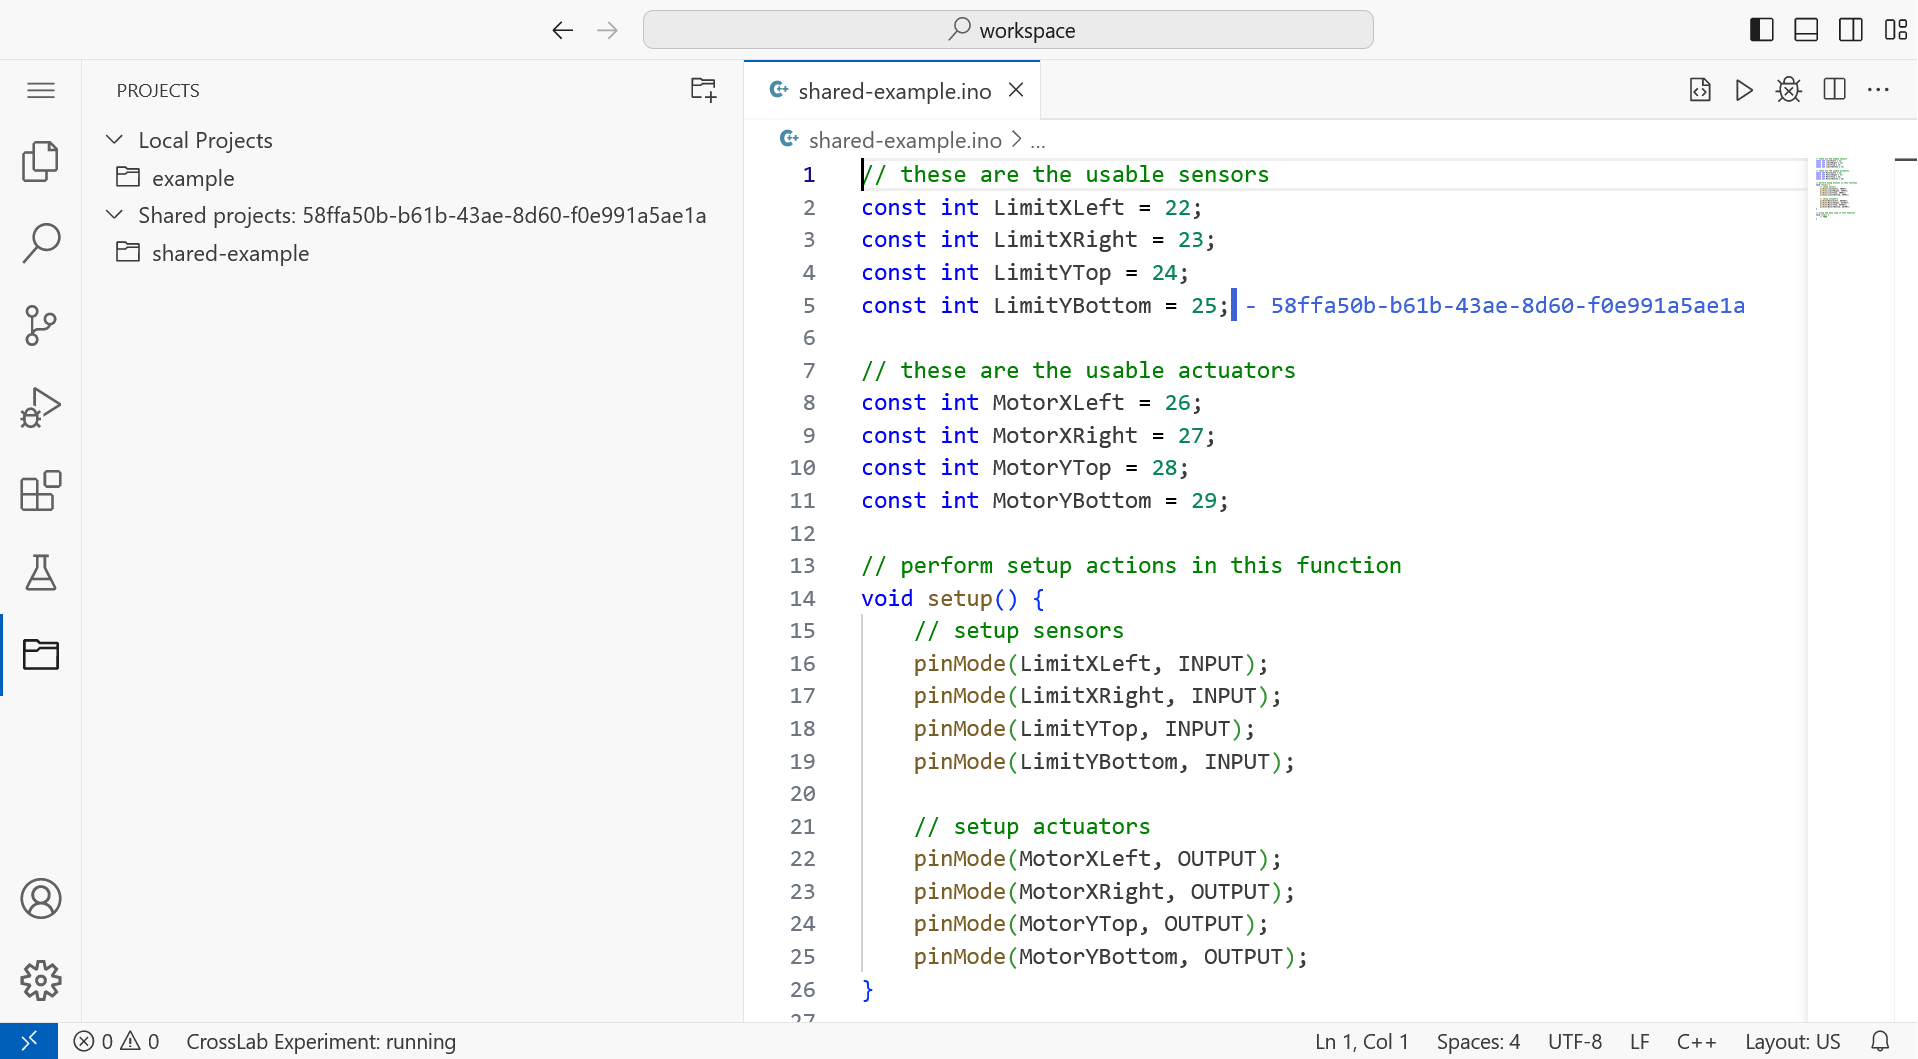
\includegraphics[trim={0 3px 0 0},clip,width=\textwidth]{images/projects-shared.png}
    \caption{Benutzerinterface der Projektverwaltung}
    \label{figure:benutzerinterface:dateisystem}
\end{figure}

Um die in \autoref{section:konzeption:dateisystem} beschriebenen Konzepte für die Bereitstellung und Nutzung von Dateisystemen umzusetzen, wurden der Filesystem Service sowie eine entsprechende Erweiterung für die IDE entwickelt. Diese Erweiterung wird im Folgenden als \textit{Filesystem Erweiterung} bezeichnet.

In \autoref{figure:klassendiagramm-dateisystem-service} ist ein Klassendiagramm für den Filesystem Service dargestellt. Der Filesystem Service Consumer besitzt die in \autoref{section:konzeption:dateisystem} genannten Funktionen zur Interaktion mit dem vom Filesystem Service Producer angebotenen Dateisystem. Der Filesystem Service Producer ermöglicht die Registrierung von Event-Handlern um auf die verschiedenen Anfragen reagieren zu können. Dadurch kann die Implementierung an das angebotene Dateisystem angepasst werden.

Die Filesystem Erweiterung ist für die Bereitstellung des integrierten Dateisystems und die Ermöglichung des kollaborativen Arbeitens an Programmen verwantwortlich. Für das integrierte Dateisystem wurde ein projektbasierter Ansatz gewählt. Dabei besitzen Nutzer mehrere verschiedene \textit{Projektordner}, deren direkte Unterordner als \textit{Projekte} bezeichnet werden. In der aktuellen Implementierung gibt es standardmäßig den Projektordner \texttt{/projects}. Die Projektordner sowie die enthaltenen Projekte werden dem Nutzer über ein entsprechendes Benutzerinterface angezeigt. Über dieses kann der Nutzer Projekte erstellen, öffnen, umbenennen und löschen. Für die Einbindung des Dateisystems wurde das Interface \texttt{FileSystemProvider} der VSCode Extension API implementiert. Für die Bereitstellung der Dateisystem-Funktionen können unterschiedliche \textit{Subprovider} verwendet werden. In der aktuellen Implementierung stehen dabei Subprovider für In-Memory, die Indexed Database API sowie den Filesystem Service zur Verfügung. Dabei werden standardmäßig der In-Memory Subprovider sowie der Indexed Database Subprovider für die persistente Speicherung der Projekte im Pfad \texttt{/projects} verwendet. Allerdings können der standardmäßig benutzte Subprovider sowie die Subprovider für bestimmte Pfade angepasst und neue Subprovider hinzugefügt werden. Weiterhin wurden auch die Schnittstellen \texttt{FileSearchProvider} und \texttt{TextSeachProvider} der VSCode Extension API implementiert, um es Nutzern zu ermöglichen, nach Dateien und Texten innerhalb des aktuellen Projekts zu suchen. Für das Benutzerinterface wurde eine \texttt{TreeView} verwendet, deren Daten über einen entsprechenden \texttt{TreeDataProvider} bereitgestellt werden. Das von der Filesystem Erweiterung bereitgestellte Benutzerinterface zur Verwaltung der Projekte ist in \autoref{figure:benutzerinterface:dateisystem} dargestellt. Dieses enthält auch bereits ein geteiltes Projekt, um die Darstellung unterschiedlicher Projektordner hervorzuheben.

Beim Öffnen eines neuen Ordners wird VSCode standardmäßig neugeladen. Dadurch werden auch alle Erweiterungen beendet und neugestartet, was dazu führt, dass das laufende Experiment beendet wird. Um dies zu vermeiden, muss der Wechsel von Projekten über einen anderen Mechanismus geschehen. Dazu wurde zunächst ein Pfad festgelegt, welcher standardmäßig von der IDE geöffnet wird. Im Falle der prototypischen Implementierung wurde der Pfad \texttt{/workspace} ausgewählt. Dieser Pfad nutzt standardmäßig einen In-Memory Subprovider. Sollte der Nutzer nun ein Projekt öffnen, wird von diesem Moment an der Pfad \texttt{/workspace} in allen URLs durch den Pfad des geöffneten Projektes ersetzt. Dadurch wird kein Neuladen der IDE ausgelöst und Nutzer können zwischen ihren Projekten wechseln. Das Umschreiben der Pfade führt allerdings zu Problemen beim Kopieren, Ausschneiden und Einfügen von Ordnern und Dateien. Daher müssen die entsprechenden Kommandos überschrieben werden, um die erwartete Funktionalität zu gewährleisten.

Um das Teilen von Projekten sowie das gleichzeitige Bearbeiten dieser zwischen Nutzern innerhalb eines Experiments zu ermöglichen, wurde eine entsprechende Komponente implementiert. Diese nutzt den \texttt{FileSystemProvider} sowie den von der Collaboration Erweiterung bereitgestellten Collaboration Service Prosumer. Über diesen wird ein enstsprechender Raum erstellt. Zu Beginn wird kein Projekt geteilt. Sobald ein Nutzer ein Projekt teilt, wird es zu dem geteilten Objekt des Raums hinzugefügt. Weiterhin werden auch Funktionen registriert, die auf Änderungen innerhalb des Projekts reagieren. Andere Nutzer die an der Kollaboration teilnehmen, können dann das geteilte Projekt über das bereitgestellte Benutzerinterface aufrufen. Alle Änderungen an Dateien und Ordnern werden zwischen den Nutzern synchronisiert. Weiterhin wird die aktuelle Position eines Nutzers innerhalb einer Datei über dessen Zustandsinformationen geteilt. Diese Position wird dann bei anderen Nutzern innerhalb derselben Datei markiert (siehe \autoref{figure:benutzerinterface:dateisystem}). Wenn der Besitzer des Projekts das Teilen beendet, wird das Projekt für alle anderen Nutzer geschlossen. Geteilte Projekte besitzen Pfade der Form \texttt{/shared/\{\{user\_id\}\}/\{\{project\_name\}\}}, wobei der Pfad \texttt{/shared} ein In-Memory Dateisystem verwendet. Die Projektordner \texttt{/shared/\{\{user\_id\}\}} werden automatisch erstellt, wenn ein Nutzer dem entsprechenden Raum beitritt.

Der betrachteten Experimentkonfiguration werden keine neuen Laborgeräte hinzugefügt. Die IDEs werden um einen Filesystem Service Consumer erweitert, der die Anbindung von weiteren Dateisystemen ermöglicht. Außerdem bieten die IDEs auch einen Filesystem Service Producer an, um die Nutzung des integrierten Dateisystems durch andere Laborgeräte zu ermöglichen (siehe \autoref{figure:experimentkonfiguration:dateisystem}). Zudem wird ein neuer Raum für die Verbindungen der Collaboration Service Prosumer hinzugefügt, um das Teilen von Projekten zu ermöglichen.
\section{Kompilierung}\label{section:prototypische-implementierung:kompilierung}

\begin{note}
    \textbf{Notizen:}
    \begin{itemize}
        \item Begründung warum Arduino CLI für die Implementierung genutzt wurde
        \item Beschreibung der Anbindung der Arduino CLI als Laborgerät
        \item (Angabe der Rückgabeformate?)
        \item Ggf. Beschreibung der Benutzerinterfaces + Screenshots
    \end{itemize}
\end{note}

Für die Kompilierung wurde in der prototypischen Implementierung das Arduino Command Line Interface \cite{noauthor_arduino-cli_nodate} verwendet. Dieses nutzt intern den Compiler \ac{GCC} \cite{noauthor_gcc_nodate}. Neben der Kompilierung des Quellcodes werden auch Arduino spezifische Vorverarbeitungsschritte durchgeführt. Dadurch können Nutzer auch ggf. ihnen bereits bekannte Arduino Funktionen wie z.B. \texttt{digitalWrite} und \texttt{digitalRead} nutzen. Im Allgemeinen sollte dadurch die Programmierung der Microcontroller für die Nutzer vereinfacht werden. Um die Arduino-cli zur Kompilierung innerhalb eines Experiments nutzen zu können muss diese als ein entsprechendes Laborgerät bereitgestellt werden. Dafür wurde ein cloud-instanziierbares Laborgerät entwickelt. Dieses bietet einen entsprechenden Kompilierungs Service Producer an, welcher während einem Experiment mit der IDE verbunden werden kann. Das instanziierte Laborgerät nimmt die entsprechenden Kompilieranfragen entgegen und bearbeitet diese. Sollte die Kompilierung erfolgreich sein wird eine entsprechende Antwort mit dem Ergebnis der Kompilierung an die IDE gesendet. Im Fehlerfall wird die Fehlermeldung in der Antwort mitgesendet.

Um die Kompilierung aus der IDE starten zu können wurde eine entsprechende Erweiterung entwickelt. Diese fügt zwei Bedienelemente hinzu. Eine Schaltfläche zur Kompilierung des aktuellen Projekts sowie eine Taste zum Kompilieren und Hochladen des aktuellen Projekts. Die erste Schaltfläche kann dazu genutzt werden um zu überprüfen ob das aktuelle Projekt kompiliert werden kann und um die entsprechenden Mitteilungen vom Compiler zu erhalten. Die zweite Schaltfläche führt auch eine Kompilierung des aktuellen Projekts durch und zeigt entsprechende Rückmeldungen an. Sollte die Kompilierung erfolgreich sein wird anschließend das Ergebnis dieser an die zu programmierende Steuereinheit gesendet. In einer kollaborativen Sitzung ist das Kompilieren von Projekten stets erlaubt. Allerdings wird das Hochladen von Projekten deaktiviert falls ein anderer Nutzer aktuell ein Projekt auf die Steuereinheit hochlädt oder falls die Steuereinheit in einer Debug-Sitzung verwendet wird.
\section{Debugging}\label{section:prototypische-implementierung:debugging}

\begin{figure}[tbp]
    \centering
    \resizebox{\textwidth}{!}{
        \begin{tikzpicture}
            \begin{class}[text width=7.5cm]{DebuggingAdapterServiceProducer}{0,0}
                \operation{+ sendMessageDAP()}
                \operation{+ onStartSession()}
                \operation{+ onJoinSession()}
                \operation{+ onMessageDAP()}
            \end{class}
            \begin{class}[text width=7.5cm]{DebuggingAdapterServiceConsumer}{8,0}
                \operation{+ sendMessageDAP()}
                \operation{+ startSession()}
                \operation{+ joinSession()}
                \operation{+ onMessageDAP()}
            \end{class}
            \begin{class}[text width=7.5cm]{DebuggingTargetServiceProducer}{0,-3.5}
                \operation{+ sendDebuggingMessage()}
                \operation{+ onStartDebugging()}
                \operation{+ onEndDebugging()}
                \operation{+ onDebuggingMessage()}
            \end{class}
            \begin{class}[text width=7.5cm]{DebuggingTargetServiceConsumer}{8,-3.5}
                \operation{+ sendDebuggingMessage()}
                \operation{+ startDebugging()}
                \operation{+ endDebugging()}
                \operation{+ onDebuggingMessage()}
            \end{class}
        \end{tikzpicture}
    }
    \caption{Klassendiagramm Debugging Services}
    \label{figure:klassendiagramm-debugging-services}
\end{figure}

Für die Bereitstellung der Debug-Funktionen wurde in der prototypischen Implementierung der \textit{\ac{GDB}} \cite{noauthor_gdb_nodate} verwendet. Dieser erlaubt das Debuggen von Microcontrollern und besitzt zudem einen integrierten Debug Adapter. Um \ac{GDB} in Experimenten nutzen zu können, wurde ein cloud-instanziierbares Laborgerät entwickelt. Dieses stellt einen Debugging Adapter Service Producer und einen Debugging Target Service Consumer für die Kommunikation mit der IDE sowie der zu debuggenden Steuereinheit bereit.

In \autoref{figure:klassendiagramm-debugging-services} ist ein Klassendiagramm für den Debugging Adapter Service und den Debugging Target Service dargestellt. Hierbei besitzt der Debugging Adapter Service Consumer die Funktionen \texttt{startSession()} und \texttt{joinSession()}, um eine neue Debug-Sitzung zu starten oder einer laufenden beizutreten. Der Debugging Adapter Service Producer löst entsprechende Events aus, die über Event-Handler behandelt werden können. Sowohl der Debugging Adapter Service Consumer als auch der Debugging Adapter Service Producer besitzen Funktionen, um DAP-Nachrichten zu versenden und auf diese zu reagieren. Der Debugging Target Service Consumer besitzt die Funktionen \texttt{startDebugging()} und \texttt{endDebugging()}, um den Beginn bzw. das Ende einer Debug-Sitzung zu signalisieren. Auch hier löst der Debugging Target Service Producer entsprechende Events aus, die über Event-Handler behandelt werden können. Sowohl der Debugging Target Service Consumer als auch der Debugging Target Service Producer besitzen Funktionen, um Debug-Nachrichten zu versenden und auf diese zu reagieren.

Wenn ein Nutzer eine Debug-Sitzung startet, wird über den Debugging Adapter Service eine entsprechende Nachricht an das Laborgerät des Debuggers gesendet. Diese Nachricht beinhaltet das aktuelle Projekt des Nutzers. Dieses benötigt der Debugger während der Debug-Sitzung, weshalb es für die Dauer der Debug-Sitzung in einem entsprechenden Ordner auf dem Dateisystem hinterlegt wird. Weiterhin wird das Projekt an den Compiler gesendet, wobei für die Ermöglichung des Debuggens spezielle Einstellungen vorgenommen werden müssen. Das Ergebnis der Kompilierung wird dann über den Debugging Target Service an die Steuereinheit gesendet, wodurch der Steuereinheit gleichzeitig der Beginn einer Debug-Sitzung mitgeteilt wird. Weiterhin wird der Debugger selbst gestartet, wobei der tatsächliche Start der Debug-Sitzung erst durch die Nachrichten des \ac{DAP} geschieht. Nachdem alle Vorbereitungen getroffen wurden und eine Antwort von der Steuereinheit empfangen wurde, wird eine Antwort an die IDE gesendet. Die Antwort enthält den Kennzeichner der Debug-Sitzung sowie Einstellungen für diese. Im Falle der prototypischen Implementierung werden hierbei der Kennzeichner der Debug-Sitzung, das Debug-Ziel sowie der Pfad des kompilierten Programms als Einstellungen übergeben. Diese werden dann von der IDE beim Start des \ac{DAP} verwendet.

Damit das \ac{DAP} korrekt ausgeführt werden kann, muss eine Umschreibung der URIs vorgenommen werden, da die Dateien des Nutzers und des Debuggers unterschiedliche URIs besitzen. Außerdem gibt es Dateien, die nur auf dem Dateisystem des Debuggers vorhanden sind, wie z.B. Bibliotheken. Alle URIs, die von der IDE gesendet werden, beginnen entweder mit \texttt{crosslabfs:/workspace} für Dateien innerhalb eines Projekts oder mit \texttt{crosslab-remote:} für Dateien innerhalb des Dateisystems des Debuggers. Bei Ersteren wird das genannte Präfix durch den lokalen Pfad des Projektes auf dem Dateisystem des Debuggers ersetzt, während bei Zweiteren das Präfix gelöscht wird. Bei Nachrichten vom Debugger an die IDE werden Dateien innerhalb des Projekts wieder auf URIs beginnend mit \texttt{crosslabfs:/workspace} abgebildet, während alle anderen Dateien das Präfix \texttt{crosslab-remote:} erhalten.

Um das kollaborative Debuggen innerhalb eines Experiments zu unterstützen, müssen einige Nachrichten des \ac{DAP} speziell behandelt werden. Dazu gehören die Nachrichten für Breakpoints, Stacktraces, das Starten und Stoppen des Programms sowie das Beenden der Debug-Sitzung. Wenn Nutzer einer Debug-Sitzung beitreten, schicken sie zunächst nur ihre lokalen Breakpoints über eine \texttt{SetBreakpoints}-Anfrage. Damit nicht die Breakpoints der anderen Nutzer gelöscht werden, müssen diese entsprechend zu dieser Nachricht hinzugefügt werden. Dafür werden die Breakpoints aller Nutzer separat verwaltet. Außerdem müssen alle Events gespeichert werden, um diese beitretenden Nutzern schicken und den aktuellen Zustand der Debug-Sitzung herstellen zu können. Allgemein werden Events, die vom Debug Adapter ausgegeben werden, an alle Nutzer einer Debug-Sitzung gesendet. Wenn ein Nutzer das Programm startet oder fortsetzt, muss ein \texttt{Continued}-Event an die anderen Nutzer gesendet werden. Bei Breakpoints und Stacktraces muss darauf geachtet werden, dass die URIs für Dateien des Debuggers entsprechend angepasst werden, damit die IDE diese öffnen kann. Wenn der Ersteller der Debug-Sitzung diese beendet, so wird sie für alle Nutzer beendet. Sollte ein anderer Nutzer die Debug-Sitzung beenden, so wird sie nur für diesen Nutzer selbst beendet.

\begin{figure}[tbp]
    \centering
    \begin{tikzpicture}
        \node[anchor=south west,inner sep=0] at (0,0) {
\includegraphics[trim={8.5cm 0 9.1cm 0},clip,width=0.1\textwidth]{images/symbols.png}};
        \node[anchor=south west,inner sep=0] at (2,0) {
\includegraphics[trim={8.5cm 0 9.1cm 0},clip,width=0.1\textwidth]{images/symbols-join.png}};
        \draw[orange,ultra thick,rounded corners] (0.2,0.2) rectangle (1.35,1.55);
        \draw[blue!60,ultra thick,rounded corners] (2.2,0.2) rectangle (3.35,1.55);
        \node[orange] at (-2.8,0.75) {Starten einer Debug-Sitzung};
        \node[blue!60] at (6.5,0.75) {Beitreten einer Debug-Sitzung};
    \end{tikzpicture}
    \caption{Schaltflächen für das Starten und Beitreten einer Debug-Sitzung}
    \label{figure:benutzerinterface:symbole-debugging}
\end{figure}

\begin{figure}[tbp]
    \centering
    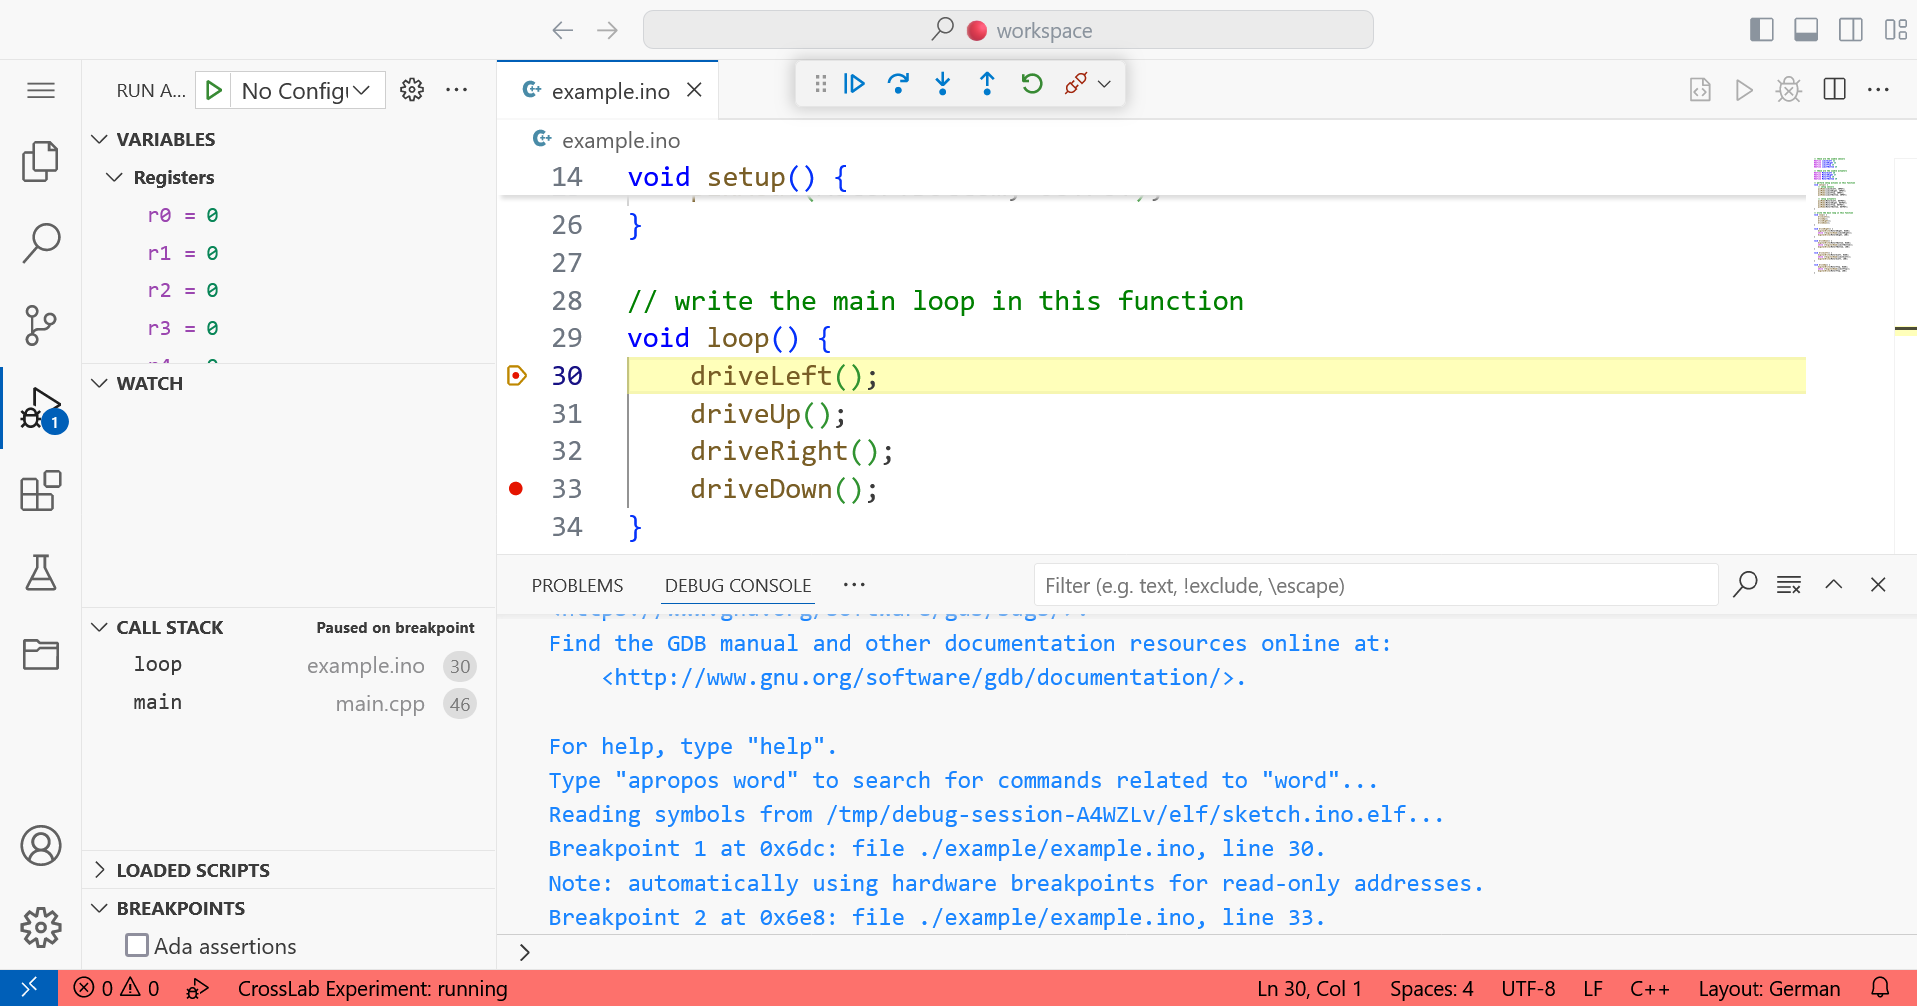
\includegraphics[trim={0 3px 0 0},clip,width=\textwidth]{images/debugging.png}
    \caption{Benutzerinterface der IDE während einer aktiven Debug-Sitzung}
    \label{figure:benutzerinterface:debugging}
\end{figure}

Für die Einbindung in die IDE wurde eine entsprechende Erweiterung entwickelt. Diese wird im Folgenden als \textit{Debugging Erweiterung} bezeichnet und fügt einen Debugging Adapter Service Consumer hinzu. Die Debugging Erweiterung beinhaltet zudem Implementierungen der Schnittstellen \texttt{DebugAdapter}, \texttt{DebugAdapterDescriptorFactory} und \texttt{DebugConfigurationProvider}. Mithilfe dieser Schnittstellen kann bereits ein Großteil der Funktionalität implementiert werden. Weiterhin werden auch Bedienelemente zum Starten bzw. Beitreten einer Debug-Sitzung bereitgestellt. Diese sind in \autoref{figure:benutzerinterface:symbole-debugging} dargestellt. Nutzer können eine Debug-Sitzung über eine entsprechende Schaltfläche starten, falls keine aktive Debug-Sitzung bestehen sollte. Ansonsten können Nutzer über eine weitere Schaltfläche einer bestehenden Debug-Sitzung beitreten, falls sie Zugriff auf das dazugehörige Projekt haben. In \autoref{figure:benutzerinterface:debugging} wird das Benutzerinterface der IDE während einer aktiven Debug-Sitzung gezeigt. Um das Debuggen von Dateien zu ermöglichen, die nur im Dateisystem des Debuggers vorhanden sind, wurde ein \texttt{TextDocumentContentProvider} implementiert. Dieser ermöglicht Lesezugriff auf die Dateien innerhalb des Dateisystems des Debuggers sowie das Setzen von Breakpoints innerhalb dieser.

Das betrachtete Experiment wird um das neue Laborgerät für die Bereitstellung von GDB erweitert. Dieses wird über den Debugging Adapter Service mit den IDEs verbunden. Außerdem wird die Steuereinheit um einen Debugging Target Service Producer erweitert. Der Debugger wird über den Debugging Target Service mit der Steuereinheit verbunden (siehe \autoref{figure:experimentkonfiguration:debugging}).
\section{Testen}\label{section:prototypische-implementierung:testen}

\begin{figure}[tbp]
    \centering
    \begin{tikzpicture}
        \begin{class}[text width=6cm]{TestingServiceProducer}{0,0}
            \operation{+ registerFunction()}
            \operation{+ onStartTesting()}
            \operation{+ onEndTesting()}
            \operation{+ onFunctionCall()}
        \end{class}
        \begin{class}[text width=6cm]{TestingServiceConsumer}{7,0}
            \operation{+ addTest()}
            \operation{+ runTest()}
            \operation{+ startTesting()}
            \operation{+ endTesting()}
        \end{class}
    \end{tikzpicture}
    \caption{Klassendiagramm Testing Service}
    \label{figure:klassendiagramm-testing-service}
\end{figure}

Für die prototypische Implementierung wurde der in \autoref{section:konzeption:testen} konzipierte Testing Service implementiert. Das Klassendiagramm für diesen kann in \autoref{figure:klassendiagramm-testing-service} eingesehen werden. Der Testing Service Producer ermöglicht es Laborgeräten mithilfe von \texttt{registerFunction()} Funktionen für die Erstellung von Testfällen bereitzustellen. Dabei sollten neben dem Namen und der Implementierung der Funktion auch Schemata für die Argumente und den Rückgabewert der Funktion angegeben werden, damit eine Validierung dieser möglich ist. Die Erstellung von Testfällen kann während der Erstellung eines Experiments vorgenommen werden. Dabei werden diese in der Konfiguration des Laborgeräts hinterlegt, welches den Testing Service Consumer anbietet. Der Testing Service Consumer kann, wie in der Konzeption beschrieben, mit \texttt{startTesting()} das Testen starten, mit \texttt{runTest()} Testfälle ausführen und mit \texttt{endTesting()} das Testen beenden. Der Testing Service Producer löst entsprechende Events aus, die über Event-Handler behandelt werden können.

\begin{figure}[tbp]
    \centering
    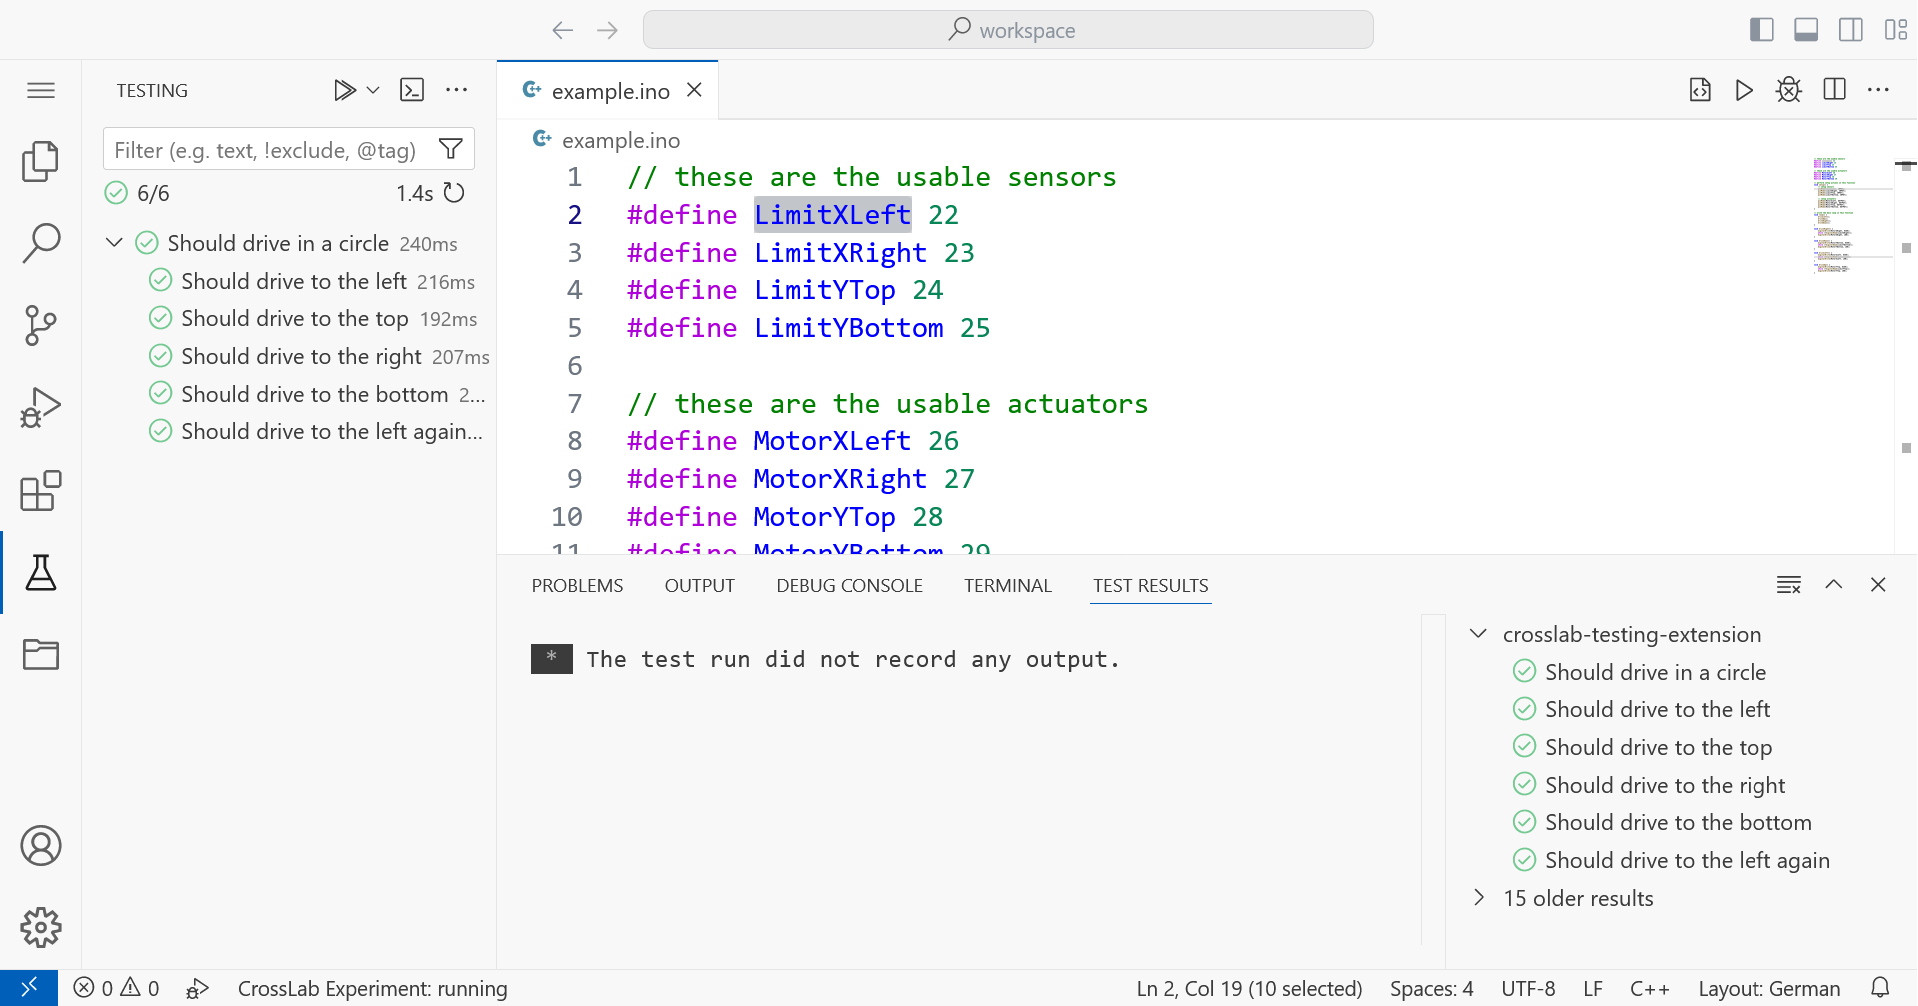
\includegraphics[trim={0 3px 0 0},clip,width=\textwidth]{images/tests-success.png}
    \caption{Benutzerinterface für die Ausführung von Testfällen}
    \label{figure:benutzerinterface:testen}
\end{figure}

Für die IDE wurde eine entsprechende Erweiterung implementiert. Diese wird im Folgenden als \textit{Testing Erweiterung} bezeichnet und stellt einen Testing Service Consumer bereit. Weiterhin wird die VSCode Testing API, ein Teil der VSCode Extension API, verwendet, um die Testfälle in der IDE anzeigen und ausführen zu können. Dabei wird das bereits in VSCode enthaltene Benutzerinterface für Tests verwendet. Dieses ist in \autoref{figure:benutzerinterface:testen} dargestellt.

Der betrachteten Experimentkonfiguration wird kein neues Laborgerät hinzugefügt. Jede IDE wird um einen Testing Service Consumer und die Steuereinheit um einen Testing Service Producer erweitert. Zudem stellt die Steuereinheit Funktionen zum Setzen und Auslesen der Pins des simulierten Microcontrollers zur Verfügung. Es werden Verbindungen zwischen den IDEs und der Steuereinheit über den Testing Service hinzugefügt (sh. \autoref{figure:experimentkonfiguration:testen}).
\section{Language Server}\label{section:prototypische-implementierung:language-server}

% \begin{note}
%     \textbf{Notizen:}
%     \begin{itemize}
%         \item Begründung warum Arduino Language Server genutzt wurde
%         \item Anbindung des Arduino Language Server als Laborgerät
%         \item Beschreibung der implementierten VSCode Erweiterung
%         \item Beschreibung der aufgetretenen Probleme und deren Lösung
%     \end{itemize}
% \end{note}

Für die prototypische Implementierung wurde ein cloud-instanziierbares Laborgerät für die Bereitstellung des \textit{Arduino Language Servers} \cite{noauthor_arduino-language-server_2025} implementiert. Dieses besitzt einen entsprechenden Language Server Service Producer. Wenn die IDE den Language Server startet, schickt sie zunächst die entsprechende Initialisierungsnachricht mit dem aktuellen Projekt des Nutzers. Dieses wird auf der Seite des Language Server gespeichert. Danach wird der Language Server gestartet und eine Antwort an die IDE gesendet. Diese kann daraufhin mit der Ausführung des \ac{LSP} beginnen. Dabei muss auf der Seite des Language Servers eine Anpassung der URIs für eingehende und ausgehende \ac{LSP} Nachrichten erfolgen. Dies kann auf eine ähnliche Weise erfolgen, wie es bereits in \autoref{section:prototypische-implementierung:debugging} für das \ac{DAP} beschrieben wurde.

Für die IDE wurde eine entsprechende Erweiterung entwickelt. Diese wird im Folgenden als \textit{Language Server Erweiterung} bezeichnet und stellt einen Language Server Service Consumer bereit. Wenn eine Verbindung für diesen besteht, wird der entsprechende Language Server gestartet und über den VSCode Language Client angebunden. Weiterhin wurde ein \texttt{TextDocumentContentProvider} implementiert, der in Verbindung mit dem Language Server Service Consumer den Lesezugriff auf die lokalen Dateien des Language Servers ermöglicht.

Die betrachtete Experimentkonfiguration wird um das neue Laborgerät für die Bereitstellung des Arduino Language Servers erweitert. Dieses wird über den Language Server Service mit den IDEs verbunden.
\chapter{Fazit und Ausblick}\label{section:fazit-und-ausblick}

% opt: zusätzliche Anhänge
\begin{appendix}
    % \input{content/anhang1}
\end{appendix}

% --- Abbildungs-, Tabellen-, Algorithmen- und Literaturverzeichnis ------------
\backmatter
% Abbildungsverzeichnis
\listoffigures
% Tabellenverzeichnis
\listoftables
% Algorithmenverzeichnis
\listofalgorithms
% Literaturverzeichnis
\cleardoublepage	% Literaturverzeichnis immer auf ungerader Seite
\phantomsection		% Anker für Sprungmarke im Inhaltsverzeichnis korrigieren
\addcontentsline{toc}{chapter}{\bibname}
\bibliography{NIKR_bibliography}
\end{document}
